\documentclass[12pt]{article}

% Packages essentiels
\usepackage[utf8]{inputenc}
\usepackage[T1]{fontenc}
\usepackage[english]{babel}
\usepackage{geometry}
\geometry{margin=2.5cm}
\usepackage{booktabs}
\usepackage{longtable}
\usepackage{ltcaption} % For better longtable captions with hyperref
\usepackage{multirow}
\usepackage{array}
\usepackage{tabularx}
\usepackage{colortbl}
\usepackage{graphicx}
\usepackage{xcolor}
\usepackage{eso-pic}
\usepackage{tikz}
\usepackage{authblk}
\usepackage{pdflscape}
\usepackage{afterpage}
\usepackage{float}

% Bibliography setup
\usepackage[backend=biber,style=authoryear,sorting=nyt]{biblatex}
\addbibresource{references.bib}

\usepackage[
  unicode=true,
  colorlinks=true,
  linkcolor=blue,
  citecolor=blue,
  urlcolor=blue
]{hyperref}
\usepackage{cleveref}

\usepackage{enotez}
\let\footnote=\endnote
\setenotez{
  list-name={Notes},
  backref=true
}


% Configure cleveref for tables in appendix
\crefname{table}{Table}{Tables}
\Crefname{table}{Table}{Tables}

% TikZ libraries for logo opacity and diagram features
\usetikzlibrary{positioning,backgrounds,fit,shapes,calc,matrix}
\usepackage{csquotes}
\usepackage{tocloft} % For customizing table of contents

% Configure tocloft for table of contents
\renewcommand{\cfttoctitlefont}{\Large\bfseries}
\setlength{\cftbeforetoctitleskip}{0pt}
\setlength{\cftaftertoctitleskip}{1em}

% Allow line breaks in \texttt at underscores
\renewcommand\_{\texttt{\detokenize{_}\allowbreak}}

\title{\textbf{CCF Database: A Machine-Learning-Preprocessed Media Corpus of 264,000 Climate Articles with 65 Sentence-Level Annotation Categories (1978–2024)}}

\author[1]{Antoine Lemor}
\author[2]{Alizée Pillod}
\author[2]{Matthew Taylor}
\affil[1]{Université de Sherbrooke}
\affil[2]{Université de Montréal}

\date{}

\begin{document}

\maketitle
\thispagestyle{empty}


\begin{abstract}
\noindent
The Canadian Climate Framing (CCF) database constitutes the largest machine-learning-preprocessed corpus of climate discourse available for research, comprising 266,271 articles from 20 Canadian newspapers (1978–2024) processed into 9.2 million sentence-level analytical units with 65 hierarchical annotations. This technical paper presents the complete methodology underlying this resource, from data collection through validation. The database addresses fundamental limitations in climate communication research by providing analysis-ready data that would otherwise require months of preprocessing and annotation. The four-phase methodology integrates systematic data collection with advanced natural language processing: (1) comprehensive article collection across bilingual sources; (2) preprocessing pipeline including deduplication, sentence segmentation, and language verification; (3) iterative human-in-the-loop machine learning training with 4,000+ expert annotations using language-specific transformer models (BERT for English and CamemBERT for French); and (4) validation and deployment, combining expert gold-standard annotation (n=1,000) with intercoder reliability assessment, achieving F1=0.866 across all categories. The hierarchical annotation framework captures eight thematic frames, nine actor types, eight event categories, two solution strategies, two emotional tones, geographic focus, and named entities, each with multiple fine-grained subcategories. Four analytical applications demonstrate the database's research potential: (1) examining how political leader mentions correlate with scientific skepticism framing; (2) mapping geographic polarization of climate science discourse across Canadian provinces; (3) testing whether thematic frames predict front-page editorial placement; and (4) constructing cocitation networks to identify epistemic authorities in climate communication. These applications show how the CCF database advances climate communication research as evidence-informed social science.
\end{abstract}

\newpage

\section{Background \& Summary}

On October 18, 1983, \textit{The Globe and Mail} ran a story headlined: “Disastrous warming of Earth to start in ’90s, report warns.” The article included the following warning:
\begin{quote}
“In the next century, [the report] warns, the world will have to learn to cope with major changes in climate patterns, with disrupted food production and with significantly higher coastal waters.”
\end{quote}
This excerpt shows that climate science has been present in Canadian media coverage for more than forty years. But more fundamentally, it tends to confirm the premise that news coverage offers a window onto social and political realities. Because most citizens do not have direct access to academic research, they rely largely on media coverage to make sense of climate change. As a result, news media occupies a central position in the climate problem: they shape not only what people think about, but also how they think about it \autocite{scheufele_framing_2007}. Beyond their impact on public opinion, media are also widely seen as influencing political agendas, even if the magnitude of this influence varies across issues and contexts \autocite{walgrave_contingency_2006}. Consequently, the media are not simply a neutral arena for public debate; they actively participate in defining and constructing the very problems under discussion \autocite{cohen_folk_1972, trevino_media_2018}.

This paper introduces the \emph{Canadian Climate Framing (CCF)} database, a machine-learning-preprocessed corpus of 266,271 climate-related newspaper articles published between 1978 and 2024 across 20 major Canadian media outlets. The dataset contains more than 9,198,158 sentences, all annotated within a 65-category hierarchical coding scheme. By focusing on Canadian print media, this study captures both a historically influential source of climate information\footnote{While digital and social media have grown in prominence over the years, newspapers remain a foundational source of information and continue to shape public discourse. Their coverage also influences other media formats  \parencite{bastos_shares_2015, casero-ripolles_impact_2020}. Focusing on print media therefore provides a vantage point on a traditional and still highly influential channel of climate communication. Crucially, analyzing newspapers allows for long-term historical comparison, including periods that predate the rise of social media.} and a uniquely complex national context\footnote{Canada offers a particularly compelling case for studying climate discourse. Its federal structure, bilingual culture, and vast territory create a microcosm of the diversity, and contradictions, found globally. While Canada is highly vulnerable to the impacts of climate change \autocite{lulham_canada_2023}, it remains significantly dependent on fossil fuel extraction and other resource-based industries \autocite{natural_resources_canada_energy_2025}. In turn, this context creates structural tensions between environmental protection and economic interests. Some of Canada's provinces, notably Quebec and British Columbia tend to adopt more progressive climate policies, whereas others with resource-intensive economies are more cautious or resistant \autocite{harrison_struggle_2010}. This combination of political decentralization, linguistic duality, and regional economic variation results in diverse policy approaches and consequently shapes how climate change is discussed in the media.}, providing, to the authors' knowledge, a rich case study  for understanding how media coverage intersects with regional, economical, linguistic, and/or political differences. 

Systematic analysis of climate communication in Canada and elsewhere has long been constrained by several methodological challenges: until recently, large-scale corpus collection and precise, reproducible content analysis were virtually impossible. Table~\ref{sec:appendix_literature} in Appendix provides an overview of prior studies in this area, highlighting the scope, focus, and coverage of existing research. The \emph{Canadian Climate Framing (CCF)} database was designed to address several of these gaps. Unlike earlier studies\footnote{Only a small number of studies have examined media coverage of climate change in the Canadian context, and those that do generally rely on a narrow set of nationally circulating newspapers—most commonly \textit{The Globe and Mail}, \textit{National Post}, and \textit{Toronto Star}. Yet, climate attitudes vary significantly across regions \autocite{hatch_what_2025}, suggesting that media coverage may also differ geographically. Nevertheless, very few studies have investigated regional climate coverage, and those that do often focus on a single province or territory rather than comparing across them. This national-level bias also produces a linguistic blind spot: in an officially bilingual country, reliance on the most widely circulated papers effectively excludes French-language media. Only two studies have examined francophone coverage in Canada—\cite{young_comparing_2012}, comparing English and French climate change media coverage, and \cite{king_how_2019}, analyzing climate change's public-health framing with partial inclusion of Quebec. A further limitation is temporal scope. Many studies examine short periods, frequently a single year, while longitudinal analyses are rare and typically cover only the late 1980s to the 2010s. As a result, most corpora remain small—often fewer than 10,000 articles—and provide limited insight into how climate discourse evolves across regions, languages, and time.}, the CCF database spans nearly five decades and draws on a larger set of newspapers, including not only nationally circulating outlets but also regional ones, thereby capturing a broader media landscape. It also better reflects Canada’s linguistic diversity through its bilingual corpus, which includes a substantial share of French-language coverage (82.9\% English, 17.1\% French).

The CCF database is the first climate media corpus to offer sentence-level annotations derived from supervised machine learning. Unlike unsupervised approaches such as topic modeling, which remain dominant in the field\footnote{Natural language processing (NLP) enables scholars to examine much larger corpora in far less time, opening new avenues for systematic inquiry \autocite{swarnakar_nlp_2021, schafer_computational_2023, hirsbrunner_computational_2024}. However, as summarized in Table 2, when climate researchers do employ NLP, it is most often to identify key actors through named entity recognition, detect stance, or conduct sentiment analysis. These applications tend only to map actors, tone, or evaluative direction rather than interpretive structures. The dominant computational approach in the field continues to be unsupervised machine learning, particularly topic modeling, where topics are treated as proxies for frames. However, as \textcite{nicholls_computational_2024} and \textcite{otmakhova_media_2024} emphasize, this assumption is problematic: topics are too narrow to capture the defining features of frames, which, following \textcite{entman_framing_1993}, require not only identifying a problem but also specifying causal interpretations, moral evaluations, and possible solutions.}, the methodology relies on transformer-based classifiers (BERT for English, CamemBERT for French) trained on over 4,000 manually expert-coded sentences. This supervised approach enables the identification of thematic frames, actor types, events, solution strategies, and emotional tone with a level of semantic precision that unsupervised methods cannot achieve. The trained models attain a macro F1 score of 0.866 across all 65 annotation categories, as validated against an independent gold standard of 1,000 expert-coded sentences whose reliability was confirmed through double-coding (Cohen's  $\kappa$ = 0.569, Krippendorff's $\alpha$ = 0.690, Gwet's AC1 = 0.893). In addition, named entity recognition (NER) was also applied to extract persons, organizations, and locations mentioned in the articles, enabling, for example, network analyses of epistemic authorities and the mapping of actor co-citation patterns across the corpus. 

Only two studies have applied comparable transformer-based models in this domain: \textcite{luo_detecting_2021} trained a single BERT classifier to analyze the evolution of partisanship in U.S. media, while \textcite{meddeb_counteracting_2022} used a CamemBERT model to detect misinformation in French news. Importantly, neither of these studies examines framing directly. More importantly, no existing research has trained and deployed such a comprehensive suite of transformer models to systematically annotate climate-related media coverage. With over 60 BERT and CamemBERT classifiers covering frames, actors, events, solutions, and emotional tone, the CCF database fills a clear methodological gap by introducing a supervised NLP approach capable of detecting multiple analytical dimensions at scale, and test numerous hypotheses. The analytical applications presented in this paper illustrate the range of research questions this resource can support, and its capacity to inform studies across diverse theoretical perspectives. 

This technical paper presents the methodology underlying the \emph{Canadian Climate Framing (CCF)} database. With its fully pre-processed, analysis-ready structure, the CCF Database constitutes the most extensive resource to date for examining Canadian climate discourse. The remainder of the document outlines the full workflow, from data acquisition and preprocessing to model training and validation, and offers the conceptual rationale and practical steps necessary for researchers wishing to work with the CCF database or adapt its methodology elsewhere.

\newpage

\section{Methods}

The CCF Database adopts a mixed-methods design that couples large-scale data collection with state-of-the-art machine learning (ML). It provides a systematic and reproducible framework for large-scale analysis of climate discourse that allows researchers to track how climate change is discussed, how narratives evolve over time, and who participates in the conversation.

Figure~\ref{fig:methodology_overview} presents the complete methodological pipeline and illustrates how the CCF Database transforms raw newspaper articles into a fully annotated database suitable for robust and reproducible climate communication research, both quantitative and qualitative. The pipeline integrates human expertise with computational methods through an iterative human-in-the-loop machine learning procedure. This approach ensured both the scalability needed to process 266,271 climate-related articles and the accuracy required for rigorous academic research.

The methodology comprises four distinct phases: (1) the \emph{Collection Phase} involved systematic gathering of climate-related articles from 20 major Canadian newspapers using search queries resulting in 266,271 articles spanning 1978–2024; (2) the \emph{Preprocessing and Design} phase transformed raw text into structured data, including sentence segmentation, language verification, and development of a comprehensive 65-category annotation framework; (3) the \emph{Machine Learning} phase created and validated transformer-based machine learning models (BERT for English, CamemBERT for French) through iterative training with over 4,000 expert manual annotations; and (4) the \emph{Validation and Deployment} phase ensured rigorous quality assurance by combining standard performance metrics with a human evaluation protocol based on an expert-coded gold standard that was independently double-coded by a second annotator to assess intercoder reliability, before deploying the trained models to annotate the complete corpus of 9.2 million sentences.

\subsection{Phase 1 \& 2: Data collection, preprocessing, database creation and annotation protocol}

\subsubsection{Step 1: Data collection}

The CCF database was built through a systematic protocol to trace the evolution of climate discourse in Canada’s bilingual print media, reaching back to the earliest available archives.

A total of 20 newspapers were selected for the analysis. The objective was to include both national and regional outlets in order to ensure broad geographic representation. Within this pool, newspapers were primarily chosen based on circulation levels \autocite{newspapers_canada_circulation_2015}, with the highest-circulating outlets retained. Additional criteria also informed the selection, including the desire to capture a range of political orientations and to build a bilingual corpus that reflects Canada’s linguistic landscape. This included French-language outlets both inside and outside Quebec, as well as one English-language outlet located in Quebec\footnote{Quebec is the only province in Canada with French as its sole official language. However, New Brunswick is officially bilingual, and several other provinces, such as northeastern Ontario along the Quebec border, also have sizeable francophone communities.}. The final selection was also partly shaped by availability constraints\footnote{For instance, when the highest-circulating newspapers were unavailable, the next highest-circulating outlets were selected. In the cases of Prince Edward Island, Nunavut and the Northwest Territories, no eligible newspapers were available for inclusion.}.

% Landscape page for methodology diagram
\begin{landscape}
\pagestyle{empty}
\vspace*{\fill}

\begin{figure}[h!]
\centering
\resizebox{0.95\linewidth}{!}{%
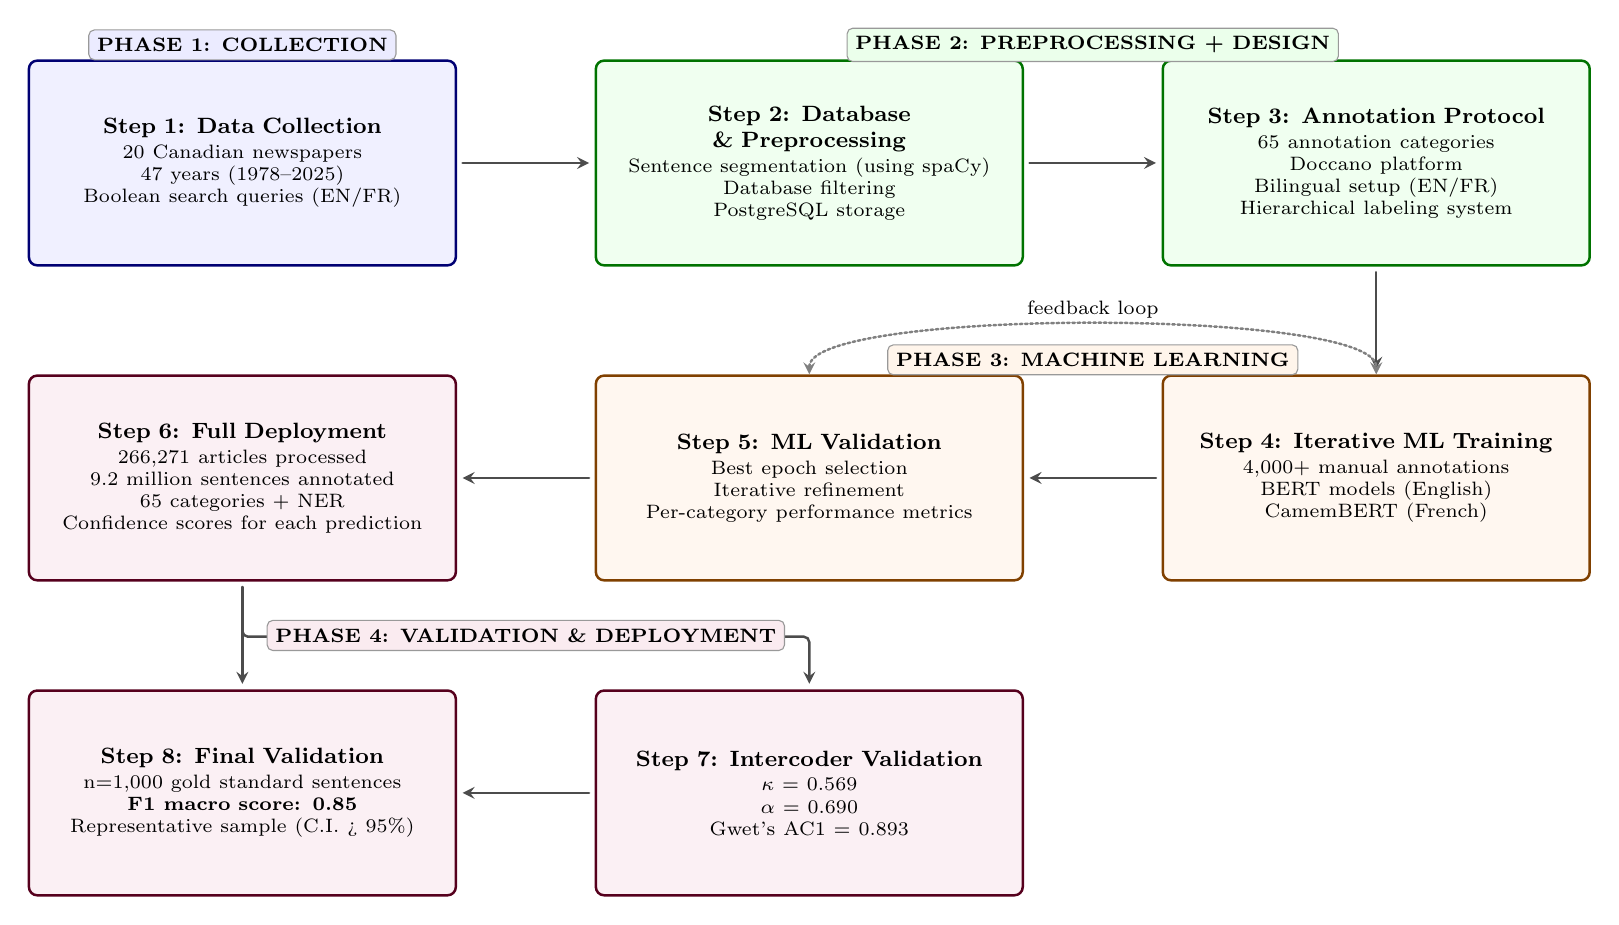
\begin{tikzpicture}[
    box/.style = {
        rectangle,
        draw=black!50,
        line width=0.9pt,
        rounded corners=3pt,
        minimum width=5.2cm,
        minimum height=2.6cm,
        align=center,
        font=\footnotesize,
        text width=5cm,
        inner sep=6pt,
        fill opacity=1
    },
    collect/.style = {box, fill=blue!6,   draw=blue!45!black},
    process/.style = {box, fill=green!6,  draw=green!45!black},
    train/.style   = {box, fill=orange!6, draw=orange!50!black},
    valid/.style   = {box, fill=purple!6, draw=purple!45!black},
    pending/.style = {box, fill=gray!6,   draw=gray!60, line width=0.9pt, dashed, text=gray!60},
    deploy/.style  = {box, fill=purple!6,    draw=purple!45!black},
    arrow/.style      = {->, line width=0.9pt, >=stealth, draw=black!70, rounded corners=2pt, shorten >=2pt, shorten <=2pt},
    dasharrow/.style  = {->, line width=0.9pt, >=stealth, draw=black!55, densely dashed, rounded corners=2pt, shorten >=2pt, shorten <=2pt},
    feedbackarrow/.style = {<->, line width=0.9pt, >=stealth, draw=black!50, densely dotted},
    phaselabel/.style = {rectangle, draw=black!40, rounded corners=2pt, inner sep=3pt, font=\scriptsize\bfseries},
    line cap=round, line join=round
]

% Define spacing
\def\hspace{7.2}
\def\vspace{4}

% Row 1: Steps 1-3
\node[collect] (datacoll) at (0,0) {
    \textbf{Step 1: Data Collection}\\[1pt]
    \scriptsize
    20 Canadian newspapers\\
    47 years (1978–2025)\\
    Boolean search queries (EN/FR)\\[1pt]
};

\node[process] (database) at (\hspace,0) {
  \textbf{Step 2: Database \& Preprocessing}\\[1pt]
  \scriptsize
  Sentence segmentation (using spaCy)\\
  Database filtering\\
  PostgreSQL storage\\[1pt]
};

\node[process] (protocol) at (2*\hspace,0) {
    \textbf{Step 3: Annotation Protocol}\\[1pt]
    \scriptsize
    65 annotation categories\\
    Doccano platform\\
    Bilingual setup (EN/FR)\\
    Hierarchical labeling system\\[1pt]
};

% Row 2: Steps 4-6 (right to left)
\node[train] (iterml) at (2*\hspace,-\vspace) {
    \textbf{Step 4: Iterative ML Training}\\[1pt]
    \scriptsize
    4,000+ manual annotations\\
    BERT models (English)\\
    CamemBERT (French)\\[1pt]
};

\node[train] (verification) at (\hspace,-\vspace) {
    \textbf{Step 5: ML Validation}\\[1pt]
    \scriptsize
    Best epoch selection\\
    Iterative refinement\\
    Per-category performance metrics\\[1pt]
};

\node[deploy] (fullannotation) at (0,-\vspace) {
    \textbf{Step 6: Full Deployment}\\[1pt]
    \scriptsize
    266,271 articles processed\\
    9.2 million sentences annotated\\
    65 categories + NER\\
    Confidence scores for each prediction\\[1pt]
};

% Row 3: Steps 7-8 (swapped positions)
\node[valid] (validation) at (0,-2*\vspace) {
    \textbf{Step 8: Final Validation}\\[1pt]
    \scriptsize
    n=1,000 gold standard sentences\\
    \textbf{F1 macro score: 0.85}\\
    Representative sample (C.I. > 95\%)\\[1pt]
};

\node[valid] (intercoder) at (\hspace,-2*\vspace) {
    \textbf{Step 7: Intercoder Validation}\\[1pt]
    \scriptsize
    $\kappa$ = 0.569\\
    $\alpha$ = 0.690\\
    Gwet's AC1 = 0.893\\[1pt]
};

% Arrows - horizontal flow in row 1
\draw[arrow] (datacoll.east) -- (database.west);
\draw[arrow] (database.east) -- (protocol.west);

% Arrows - down from row 1 to row 2
\draw[arrow] (protocol.south) -- (iterml.north);

% Arrows - horizontal flow in row 2 (right to left)
\draw[arrow] (iterml.west) -- (verification.east);
\draw[arrow] (verification.west) -- (fullannotation.east);

% Feedback loop - properly above the boxes
% Feedback loop — connect exactly at node tops, with smooth arch
\draw[feedbackarrow]
    (verification.north) to[out=90,in=90, looseness=0.3]
    node[above, yshift=1pt, font=\scriptsize, fill=white, inner sep=1pt] {feedback loop}
    (iterml.north);

% Arrows - down to row 3
\draw[arrow] (fullannotation.south) -- (validation.north);
\draw[arrow] (fullannotation.south) -- ++(0,-0.7) -| (intercoder.north);
\draw[arrow] (intercoder.west) -- (validation.east);

% Phase labels (muted colors, clearer grouping)
\node[phaselabel, fill=blue!8]   at (0,1.5)               {PHASE 1: COLLECTION};
\node[phaselabel, fill=green!8]  at (1.5*\hspace,1.5)     {PHASE 2: PREPROCESSING + DESIGN};
\node[phaselabel, fill=orange!8] at (1.5*\hspace,-2.5)    {PHASE 3: MACHINE LEARNING};
\node[phaselabel, fill=purple!8] at (0.5*\hspace,-1.5*\vspace)    {PHASE 4: VALIDATION \& DEPLOYMENT};

\end{tikzpicture}
}
\caption{Methodological pipeline of the Canadian Climate Framing (CCF) project.}
\label{fig:methodology_overview}
\end{figure}
\vspace*{\fill}

\end{landscape}

The corpus spans 47 years, from 1978 to 2024, with 1978 marking the earliest article identified. To identify climate-related articles, the authors developed comprehensive Boolean search queries tailored to each language (Table~\ref{tab:boolean_queries}). The selected queries included a variety of terms related to the climate crisis. They were extensively tested beforehand to ensure optimal performance in capturing relevant articles. To be included in the data set, an article had to contain at least one of these keywords in its title or body. These queries yielded an initial corpus of over 300,000 articles. 

\begin{center}
\begingroup
\refstepcounter{table}\label{tab:boolean_queries}
\begin{minipage}{0.95\linewidth}
\centering
\setlength{\tabcolsep}{8pt}
\renewcommand{\arraystretch}{1.25}
\textbf{Table \thetable. Boolean queries used for article retrieval}
\vspace{0.5em}

{\fontsize{10}{12}\selectfont
\begin{tabular}{>{\raggedright\arraybackslash}p{2.8cm} >{\raggedright\arraybackslash}p{12cm}}
\toprule
\textbf{Language} & \textbf{Boolean Query} \\
\midrule
English & "global warming" OR "climate change" OR "climate disruption" OR "climate disturbance" OR "climate disturbances" OR "climate crisis" OR "greenhouse gas" \\
French & "réchauffement climatique" OR "réchauffement planétaire" OR "changement climatique" OR "changements climatiques" OR "dérèglement climatique" OR "crise climatique" OR "gaz à effet de serre" \\
\bottomrule
\end{tabular}
}
\end{minipage}
\endgroup
\end{center}

\subsubsection{Step 2: Preprocessing}

The preprocessing phase transformed the raw data into a structured dataset suitable for machine learning. Each article was segmented into two-sentence contexts using language-specific spaCy models\footnote{en\_core\_web\_lg was employed for English text and fr\_dep\_news\_trf for French text, both optimized for news content processing.}. Sliding windows with single-sentence overlaps were implemented to ensure complete coverage while maintaining semantic continuity throughout each article. The choice to use two-sentence units was guided by several considerations. This level of granularity supports machine-learning applications by increasing the size of the training dataset. More importantly, working at the (near-)sentence level is the only approach that allows ex-post analysis that is highly precise and granular, because the unit of analysis is reduced to sentences rather than paragraphs, which in turn allows us to derive article-level variables by aggregating sentence-level annotations.

Quality control measures were applied systematically throughout the data preparation pipeline. Duplicate articles were identified and removed with fuzzy string-similarity algorithms set to a 95\% threshold. Any article containing less than 100 words were also removed  to eliminate reader letters, which often did not provide enough material to identify the presence of a frame and did not qualify as a press article per se. However, all other types of text (opinion columns, letters to the editor, news articles, editorials, etc.) were retained.\footnote{Regarding this matter, \textcite{lawrence_framing_2004} explains that it is precisely in editorials, or more generally in opinion texts, where journalistic standards are applied with a greater degree of flexibility, that the battle of framing is best observed.} 

Articles published by external news agencies as well (for example, \textit{Agence France-Presse},\textit{ CanWest News Service},\textit{ Reuters},\textit{ Bloomberg}) or by other newspapers not included in the analysis but which often belong to the same media conglomerate as the ones that were  selected (for example,\textit{ the }\textit{Financial Post}) were also retained. These republications align with the editorial direction of the concerned news outlet, and a republication does not contradict the objectives of the study since it indicates editorial interest in a topic concerning climate change. This process reduced the corpus to 266,271 unique articles\footnote{Duplicates of the same article from different media outlets were retained to enable the measurement of media bubbles.}. Language was verified with fastText\footnote{fastText is an open-source library by Facebook AI Research for text classification and word representations; its pre-trained language identification model detects the language of a text with high accuracy. See \url{https://fasttext.cc/}.} to ensure accurate categorization of bilingual content, and dates were standardized and performed UTF-8 normalization. This data preparation produced a clean, standardized corpus ready for machine learning and annotation, which were stored in two PostgreSQL tables: one with full metadata (including titles, main text, authors, dates, and page numbers) and another with the processed text data (including sentence segments and their corresponding IDs).

The resulting database is illustrated in Figure~\ref{fig:media_dist}, which displays the distribution of article counts by media (20 outlets), while Figure~\ref{fig:year_counts} shows total article counts per year across the full time span untill 2024\footnote{Data extraction concluded in February 2025; consequently, 2025 was excluded from the yearly counts because the year is incomplete. Nevertheless, the authors plan to update the database regularly and create an observatory.}. Finally, Figure~\ref{fig:province_dist} presents the distribution of articles by province, based on the primary location of each newspaper. This geographic breakdown shows the representativeness of the database across Canada (with 17.1\% of French articles, and 82.9\% of English articles). Three national newspapers are omitted from the provincial breakdown due to their pan-Canadian scope; nevertheless, they account for 36.2\% of the articles: The Globe and Mail, the National Post, and the Toronto Star.

\begin{figure}[!htbp]
  \centering
  \begin{minipage}[c]{0.48\textwidth}
    \centering
    \includegraphics[width=\linewidth]{../Results/Outputs/Figures/articles_by_media.png}
    \caption{Distribution of articles by media.}
    \label{fig:media_dist}
      \end{minipage}
  \hspace{0.02\textwidth}
  \begin{minipage}[c]{0.48\textwidth}
    \centering
    \includegraphics[width=\linewidth]{../Results/Outputs/Figures/articles_by_year.png}
    \caption{Total number of articles per year.}
    \label{fig:year_counts}
      \end{minipage}
\end{figure}

\begin{figure}[!htbp]
  \centering
  \includegraphics[width=0.8\textwidth,keepaspectratio]{../Results/Outputs/Figures/articles_by_province.png}
  \caption{Distribution of articles by province.}
  \label{fig:province_dist}
  \end{figure}

\subsubsection{Step 3: Annotation protocol}

The annotation framework constitutes the conceptual core of the CCF database. It comprises 65 categories organized into a hierarchical taxonomy designed to capture multiple dimensions of climate discourse at near-sentence granularity. The framework was developed through a combined theory-driven and data-driven procedure: it draws on established scholarship in framing, agenda-setting, climate communication, and social problems studies, while also being refined inductively through iterative engagement with the corpus and extensive pretesting. The full taxonomy and operational definitions are reported in Appendix~\ref{sec:appendix} (Table~\ref{tab:complete_framework}), while Table~\ref{tab:framework_summary} provides a compact overview of the framework's structure. Concretely, the framework is organized around \emph{Primary  Categories} that correspond to broad analytical dimensions, and \emph{Sub-categories} that capture internal distinctions within each \emph{Primary Categories} (Table~\ref{tab:framework_summary}). 

{\bfseries{Primary categories.}} The framework is organized around four primary analytic categories that structure the annotation protocol: \emph{Thematic Frames}, \emph{Actors/Messengers}, \emph{Events}, and \emph{Solutions} (Table~\ref{tab:framework_summary}). This design choice reflects a central insight of climate communication research: media discourse does not only describe climate change, but systematically selects interpretive lenses, attributes voice and credibility to specific actors, and connects the issue to episodic events and to (often contested) courses of action.

First, for \emph{Thematic Frames}, we build on the general framing tradition often associated with \textcite{entman_framing_1993}, which encompasses four dimensions: problem definition, causal interpretation, moral evaluation, and treatment recommendations. In practice, however, applying this framework to climate discourse presents significant challenges. Individual statements frequently span multiple dimensions, and "treatments" (i.e., proposed policy responses) prove particularly difficult to identify consistently \autocite{grundmann_using_2022}. This difficulty is amplified by the nature of climate change as a ``wicked problem,'' where proposed solutions remain subject to scientific uncertainty and political contestation \autocite{grundmann_climate_2016}. For these reasons, many studies do not apply Entman's four dimensions strictly \autocite{stede_climate_2021}. The CCF framework addresses these challenges by operationalizing thematic frames around major societal domains in which climate change is repeatedly interpreted in media discourse: economic, security, public health, cultural, environmental, political, scientific, and justice spheres (Table~\ref{tab:framework_summary}). This domain-based approach retains core elements of problem definition, causal interpretation, moral evaluation, and treatment recommendations where they naturally emerge in the data.

\begin{table}[b!]
\centering
\caption{The CCF annotation framework: 65 hierarchical categories for comprehensive climate discourse analysis}
\label{tab:framework_summary}
\footnotesize
\begin{tabularx}{\textwidth}{lcX}
\toprule
\rowcolor{gray!15}
\textbf{Main Category} & \textbf{N}$^a$ & \textbf{Sub-categories and Detection Elements} \\
\midrule
\multicolumn{3}{l}{\cellcolor{gray!10}\textbf{\textit{Primary Categories: Thematic Frames (8 frames with 35 sub-categories)}}} \\
\midrule
\textbf{Economic} & 6 & Negative/positive impacts, costs/benefits of action, sector footprint, general link \\
\textbf{Health} & 5 & Negative/positive impacts, co-benefits, healthcare footprint, general link \\
\textbf{Security} & 5 & Military response, base disruption, displacement, conflicts, defense footprint \\
\textbf{Justice} & 5 & Winners/losers, North-South responsibility, legitimacy, litigation, general link \\
\textbf{Political} & 3 & Policy measures, political debate \& opinion, general link \\
\textbf{Scientific} & 3 & Controversy, discovery \& innovation, general link \\
\textbf{Environmental} & 3 & Habitat loss, species loss, general biodiversity link \\
\textbf{Cultural} & 5 & Art, events, Indigenous practices, cultural footprint, general link \\
\midrule
\multicolumn{3}{l}{\cellcolor{gray!10}\textbf{\textit{Primary Categories: Actors, Events and Solutions (with 15 sub-categories)}}} \\
\midrule
\textbf{Actors/Messengers} & 9 & Scientists, politicians, activists, medical/economic/security/legal/cultural experts, any messenger \\
\textbf{Events} & 6 & Natural disasters, conferences, reports, elections, policy announcements, any event \\
\textbf{Solutions} & 3 & Mitigation, adaptation, any solution mention \\
\midrule
\cellcolor{gray!10}\textbf{Emotional Tone} & \cellcolor{gray!10}3 & \cellcolor{gray!10}Positive (hope, optimism), Negative (fear, anxiety), Neutral/none \\
\midrule
\cellcolor{gray!10}\textbf{Geographic Focus} & \cellcolor{gray!10}1 & \cellcolor{gray!10}Canadian places, actors, data, and policies \\
\midrule
\cellcolor{gray!10}\textbf{Urgency to act} & \cellcolor{gray!10}1 & \cellcolor{gray!10}Conveys immediate danger, crisis, or ``code red'' urgency \\
\midrule
\cellcolor{gray!10}\textbf{Named Entities} & \cellcolor{gray!10}3 & \cellcolor{gray!10}Persons (PER), Organizations (ORG), Locations (LOC) \\
\midrule
\multicolumn{3}{l}{\cellcolor{gray!25}\textbf{Total: 65 categories}} \\
\bottomrule
\end{tabularx}
\vspace{-0.1em}
{\footnotesize $^a$The \emph{N} count includes detection of the main category plus its sub-categories. For example: Economic frame detection + 5 sub-categories = 6.}
\end{table}

Second, the framework treats \emph{Solutions} as a distinct primary family rather than embedding them inside each thematic frame. This choice reflects both the empirical ambiguity of policy prescriptions in climate coverage and the substantive interest in distinguishing mitigation from adaptation, the latter having historically received less media attention \autocite{ford_coverage_2015}. Third, the \emph{Actors/Messengers} family is grounded in the long-standing finding that \emph{who} speaks about climate change matters for credibility, salience, and persuasion \autocite{trumbo_constructing_1996, boykoff_who_2011}. Finally, the \emph{Events} family reflects agenda-setting scholarship showing that media attention is cyclical and often driven by external shocks and institutional moments (e.g., disasters, major conferences, reports) \autocite{downs_up_1972, liu_explaining_2011}. Together, these four primary categories provide a theory-informed structure for capturing how climate change is framed, who is authorized to speak, what triggers attention, and which actions are articulated (Table~\ref{tab:framework_summary}).

{\bfseries{Operationalization: hierarchical taxonomy and sub-categories.}} Operationally, the framework implements a hierarchical labeling logic that mirrors its conceptual structure (Table~\ref{tab:framework_summary}). Each \emph{Primary Category} contains (i) a detection-level category that captures whether the broader dimension is present in a two-sentence unit, and (ii) fine-grained sub-categories that specify which internal distinctions apply when the primary category is detected. This design enables multi-label annotation: multiple frames, actors, events, and solutions may co-occur within the same unit, and the same applies to sub-categories. Within \emph{Thematic Frames}, each domain frame (e.g., Economic, Health, Justice) is paired with sub-categories that capture recurring interpretive distinctions observed in the literature and in the corpus (Table~\ref{tab:framework_summary}). Importantly, these sub-categories are not treated as mutually exclusive: a unit may simultaneously describe, for instance, the negative economic impacts of climate change and the economic benefits of climate action. The same principle applies to \emph{Actors/Messengers}, where a single person may legitimately be coded as multiple expert types (e.g., a physician quoted about climate-health links may also be a natural scientist). For full category definitions,  see Appendix~\ref{sec:appendix}, Table~\ref{tab:complete_framework}.

{\bfseries{Other dimensions: context, tone, urgency, and entity extraction.}} In addition to the four \emph{Primary Categories}, the framework includes theoretically motivated dimensions that capture context and meaning-making beyond framing in the strict sense (Table~\ref{tab:framework_summary}). A \emph{Geographic Focus} category records whether coverage situates climate change in a Canadian context, reflecting concerns that climate change is often portrayed as geographically distant \autocite{moser_reflections_2016}. An \emph{Emotional Tone} category captures positive, negative, or neutral valence, consistent with research showing that emotions shape how audiences interpret and respond to climate discourse \autocite{salama_role_2018, nabi_framing_2018}. An \emph{Urgency to act} category captures alarmist or ``code red'' signals that communicate immediacy and crisis framing. Finally, Named Entity Recognition (NER) extracts and classifies \emph{Persons}, \emph{Organizations}, and \emph{Locations} into a JSON field, enabling downstream analyses such as cocitation networks and the mapping of epistemic authorities (Table~\ref{tab:framework_summary}; Appendix~\ref{sec:appendix}, Table~\ref{tab:complete_framework}).

{\bfseries{Pretesting and iterative refinement.}} Finally, allongside these theoretical design choices, the framework was iteratively refined through inductive coding rounds. As sentences were annotated, emergent themes sometimes prompted targeted additions and clarifications to category definitions, followed by pretesting to ensure internal consistency and coder interpretability. This procedure strengthened the framework’s construct validity and ensured that the final taxonomy remained both theoretically anchored and empirically adequate.The following real example from the database—an excerpt from a 2022 article—illustrates the corresponding manual annotation protocol:

\begin{figure}[H]
\centering
\fcolorbox{gray!60}{gray!5}{
  \begin{minipage}{0.96\linewidth}
    \small
    \textbf{Example (annotated sentence).}\\[0.3em]
    \emph{``In Scientific American, professor of Environmental Studies at Humboldt State University Sarah Jaquette Ray writes, `Climate anxiety can operate like white fragility, sucking up all the oxygen in the room and devoting resources toward appeasing the dominant group.' But it would be a mistake to conclude that this term isn't applicable in the Global South, period.''}\\[0.6em]
    \begin{tabularx}{\linewidth}{@{}lX@{}}
      \toprule
      \textbf{Tagged Dimensions} & \textbf{Tagged categories} \\
      \midrule
      Actors/Messengers & Scientists \\
      Thematic frames & Justice (primary category) + North--South responsibility; Health (primary category) \\
      Emotional tone & Negative \\
      \bottomrule
    \end{tabularx}
  \end{minipage}
}
\end{figure}

\subsection{Phase 3: Machine learning}

The development of the training data followed an iterative manual annotation protocol aligned with the annotation framework previously described. A single expert annotator (climate policy and communication) labeled sentences in sequential batches (first 1,000 sentences, then three additional batches of 1,000 each) for a total of 4,000 annotated samples. The batching served two explicit objectives: (1) to iteratively improve and stabilize the annotation guidelines after each round; and (2) to progressively monitor and optimize model training to reach the highest attainable F1 score. This process culminated in a macro F1 score of 0.826 (see Table~\ref{tab:performance}) during the training phase (see Table~\ref{tab:complete_training_metrics} in Appendix~\ref{sec:appendix} for detailed metrics).

The sampling process drew equally from English and French language groups, with final annotation counts reaching 1,927 English and 2,073 French sentences. The training dataset was subsequently partitioned using stratified random sampling to create training (80\%) and validation (20\%) databases for each category and language. Table~\ref{tab:training_distribution} in Appendix~\ref{sec:appendix} provides the complete distribution of training and validation samples for all annotation categories. The random sampling approach ensured broad coverage across the temporal span and diverse media sources. The annotation protocol was developed with detailed operational definitions for each of the 65 categories to ensure consistency.

The machine learning pipeline leveraged transformer architectures optimized for each language through a custom fork of the AugmentedSocialScientist library \autocite{do_augmented_2022, lemor_antoinelemoraugmentedsocialscientistfork_2025}. The fork built from \textcite{do_augmented_2022} adds several functionnalities that are central to ensure robust machine learning training (metric logging at every training epoch, best-model selection using a weighted F1 score (0.7 × F1-positive + 0.3 × macro-F1), and an automated reinforced training protocol for underperforming models (described below) \autocite{lemor_antoinelemoraugmentedsocialscientistfork_2025}). English text processing employed BERT-base-uncased, while French text utilized CamemBERT-base, both containing 110 million parameters. The training strategy implemented hierarchical classification, where detection models were trained first as binary classifiers on the full annotated dataset, followed by sub-classification models trained exclusively on manually annotated sentences that were positive for the corresponding primary category. This approach minimized false positive propagation and allowed for specialized optimization for each classification task.

\begin{table}[b!]
\centering
\caption{Model training performance metrics for primary annotation categories}
\label{tab:performance}
\small
\begin{tabular}{l|rr|rr|rr}
\toprule
\rowcolor{gray!10}
\textbf{Category} & \multicolumn{2}{c}{\textbf{F1 (Class 1)}} & \multicolumn{2}{c}{\textbf{F1 (Class 0)}} & \multicolumn{2}{c}{\textbf{Macro F1}} \\
\cline{2-7}
\rowcolor{gray!10}
& \textbf{EN} & \textbf{FR} & \textbf{EN} & \textbf{FR} & \textbf{EN} & \textbf{FR} \\
\midrule
\rowcolor{gray!10}
\multicolumn{7}{l}{\textit{Thematic Frames}} \\
\midrule
Economic Frame & 0.745 & 0.814 & 0.944 & 0.957 & 0.845 & 0.885 \\
Health Frame & 0.800 & 0.667 & 0.989 & 0.994 & 0.894 & 0.830 \\
Security Frame & 0.870 & 0.800 & 0.996 & 0.997 & 0.933 & 0.898 \\
Justice Frame & 0.719 & 0.717 & 0.975 & 0.981 & 0.847 & 0.849 \\
Political Frame & 0.808 & 0.774 & 0.897 & 0.888 & 0.853 & 0.831 \\
Scientific Frame & 0.784 & 0.702 & 0.953 & 0.962 & 0.869 & 0.832 \\
Environmental Frame & 0.842 & 0.625 & 0.989 & 0.980 & 0.915 & 0.802 \\
Cultural Frame & 0.773 & 0.833 & 0.986 & 0.993 & 0.879 & 0.913 \\
\midrule
\rowcolor{gray!10}
\multicolumn{7}{l}{\textit{Other Primary Categories: Actors, Events and Solutions}} \\
\midrule
Presence of Messengers & 0.912 & 0.929 & 0.904 & 0.915 & 0.908 & 0.922 \\
Presence of Events & 0.794 & 0.819 & 0.935 & 0.932 & 0.865 & 0.876 \\
Presence of Solutions & 0.737 & 0.878 & 0.914 & 0.944 & 0.825 & 0.911 \\
Mention of Canada & 0.942 & 0.964 & 0.968 & 0.980 & 0.955 & 0.972 \\
Urgency to act & 0.760 & 0.690 & 0.987 & 0.981 & 0.874 & 0.835 \\
\midrule
\rowcolor{gray!15}
\textbf{Overall Average}* & \textbf{0.769} & \textbf{0.739} & \textbf{0.905} & \textbf{0.909} & \textbf{0.837} & \textbf{0.816} \\
\rowcolor{gray!15}
\textbf{Combined (ALL)} & \multicolumn{2}{c}{\textbf{0.754}} & \multicolumn{2}{c}{\textbf{0.907}} & \multicolumn{2}{c}{\textbf{0.826}} \\
\bottomrule
\end{tabular}

\vspace{0.3em}
\noindent\footnotesize
*Overall average across all active annotation categories (see Table~\ref{tab:complete_training_metrics} for complete metrics).
\end{table}

Models failing to achieve positive-class F1 scores above 0.70 during the training phase underwent an automated reinforced training protocol\footnote{This protocol was necessary for 15 underperforming models, primarily in abstract conceptual categories such as cultural and justice sub-frames.}. The reinforced phase implemented weighted random sampling to oversample minority classes, doubled batch size to 64, reduced learning rate to 1e-5, and applied weighted cross-entropy loss with emphasis on the positive class. This reinforcement protocol, extending training for an additional 20 epochs, successfully improved mean F1 scores by 0.23 across affected models, and managed to bring most categories above the acceptable performance threshold. However, five categories could not be trained due to insufficient annotations in the training data and were consequently excluded from the annotation framework\endnote{\textit{carbon footprint of the health sector}, \textit{positive impacts of climate change on health}, \textit{post-disaster military assistance}, \textit{Disruption of military operations due to climate change}, and \textit{carbon footprint of the defense sector}.}

\subsection{Phase 4: Deployment}

The full deployment phase applied all the trained models to annotate the complete CCF Database of 9.2 million sentences across 266,271 articles. A hierarchical classification strategy was implemented that directly mirrors the annotation protocol's structure of primary categories and their associated sub-categories, as illustrated in Figure~\ref{fig:hierarchical_annotation}. 

The hierarchical approach reflects the conceptual organization of the annotation framework with eleven primary detection categories, each with specific sub-categories. The eight thematic frames (\emph{Economic}, \emph{Health}, \emph{Security}, \emph{Justice}, \emph{Political}, \emph{Scientific}, \emph{Environmental}, and \emph{Cultural Frame}) function as primary categories with their internal distinctions—for example, \emph{Economic Frame}, when positive (=1), triggers six economic sub-models (\emph{negative/positive economic impacts of climate change}, \emph{economic disadvantages/benefits of climate action}, \emph{carbon footprint of the economic sector}), while a negative detection (=0) bypasses these entirely. 

\begin{figure}[b!]
\centering
\resizebox{0.95\textwidth}{!}{%
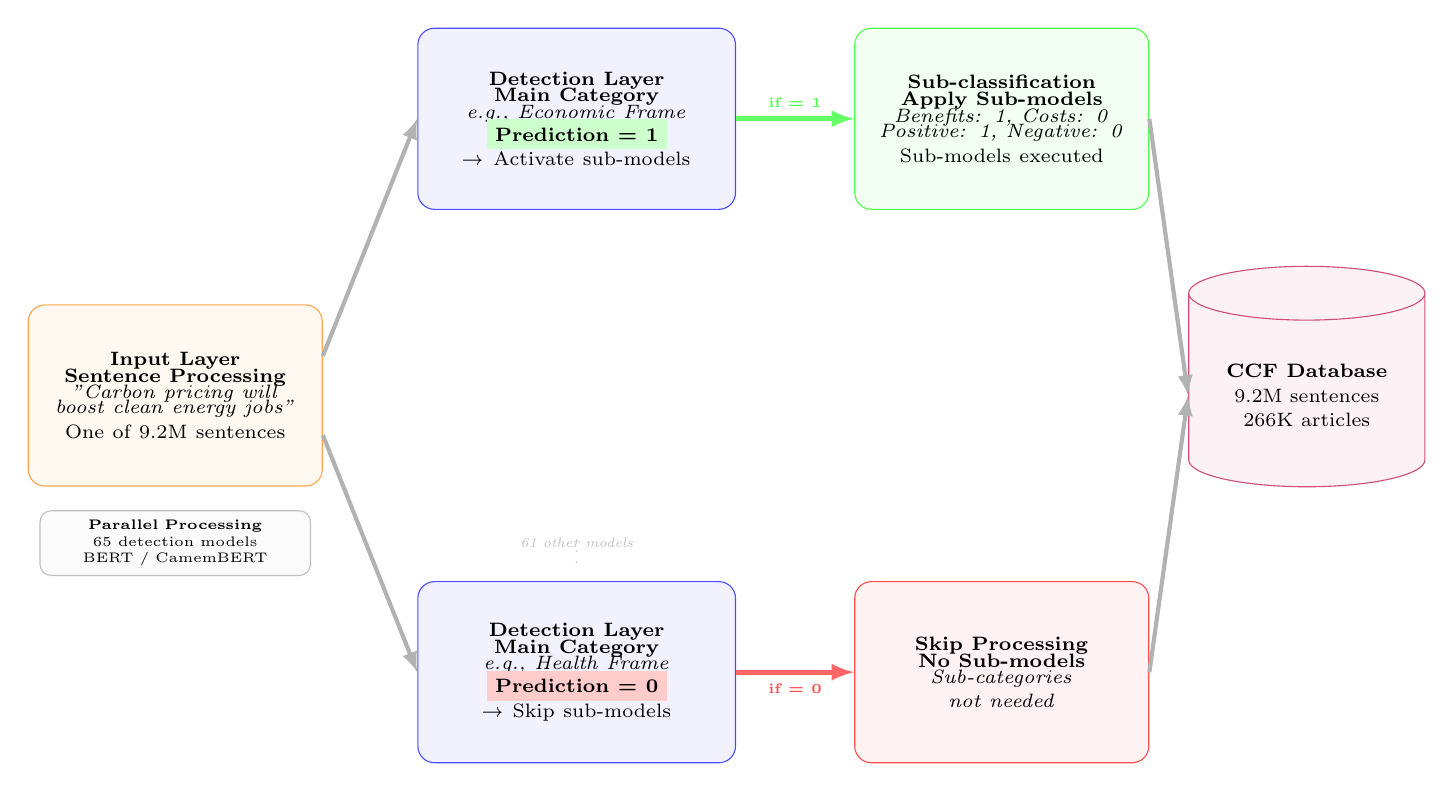
\begin{tikzpicture}[
    % Style definitions with reduced widths
    stage/.style={rectangle, rounded corners=6pt, minimum height=2.3cm, text width=3.8cm, align=center, font=\small},
    input/.style={stage, draw=orange!70, fill=orange!5, text width=3.5cm},
    detect/.style={stage, draw=blue!70, fill=blue!5, text width=3.8cm},
    process/.style={stage, draw=green!70, fill=green!5, text width=3.5cm},
    skip/.style={stage, draw=red!70, fill=red!5, text width=3.5cm},
    storage/.style={cylinder, draw=purple!70, fill=purple!5, shape border rotate=90, minimum height=2.8cm, minimum width=3cm, align=center, font=\small, aspect=0.3},
    arrow/.style={->, >=latex, line width=1.5pt, color=gray!60},
    yes/.style={arrow, color=green!60},
    no/.style={arrow, color=red!60},
    label/.style={font=\tiny\bfseries}
]

% Stage 1: Input
\node[input] (input) {
    \scriptsize\textbf{Input Layer}\\[-2pt]
    \scriptsize\textbf{Sentence Processing}\\[-2pt]
    \textit{\scriptsize "Carbon pricing will}\\[-2.5pt]
    \textit{\scriptsize boost clean energy jobs"}\\[-2pt]
    \scriptsize{One of 9.2M sentences}
};

% Stage 2: Detection (parallel branches)
\node[detect, above right=1.2cm and 1.2cm of input] (detect_yes) {
    \scriptsize\textbf{Detection Layer}\\[-2pt]
    \scriptsize\textbf{Main Category}\\[-2pt]
    \textit{\scriptsize e.g., Economic Frame}\\[-2pt]
    \colorbox{green!20}{\scriptsize\textbf{Prediction = 1}}\\[-2pt]
    \scriptsize{→ Activate sub-models}
};

\node[detect, below right=1.2cm and 1.2cm of input] (detect_no) {
    \scriptsize\textbf{Detection Layer}\\[-2pt]
    \scriptsize\textbf{Main Category}\\[-2pt]
    \textit{\scriptsize e.g., Health Frame}\\[-2pt]
    \colorbox{red!20}{\scriptsize\textbf{Prediction = 0}}\\[-2pt]
    \scriptsize{→ Skip sub-models}
};

% Stage 3: Conditional execution
\node[process, right=1.5cm of detect_yes] (execute) {
    \scriptsize\textbf{Sub-classification}\\[-2pt]
    \scriptsize\textbf{Apply Sub-models}\\[-2pt]
    \textit{\scriptsize Benefits: 1, Costs: 0}\\[-2.5pt]
    \textit{\scriptsize Positive: 1, Negative: 0}\\[-2pt]
    \scriptsize{Sub-models executed}
};

\node[skip, right=1.5cm of detect_no] (bypass) {
    \scriptsize\textbf{Skip Processing}\\[-2pt]
    \scriptsize\textbf{No Sub-models}\\[-2pt]
    \textit{\scriptsize Sub-categories}\\[-2.5pt]
    \textit{\scriptsize not needed}
};

% Stage 4: Storage - positioned at center between execute and bypass
\node[storage] (database) at ($(execute.east)!0.5!(bypass.east) + (2cm,0)$) {
    \scriptsize\textbf{CCF Database}\\[-2pt]
    \scriptsize 9.2M sentences\\[-2.5pt]
    \scriptsize 266K articles
};

% Connections
\draw[arrow] (input.15) -- (detect_yes.west);
\draw[arrow] (input.-15) -- (detect_no.west);

\draw[yes, line width=1.8pt] (detect_yes) -- node[above, label] {\textcolor{green!70}{if = 1}} (execute);
\draw[no, line width=1.8pt] (detect_no) -- node[below, label] {\textcolor{red!70}{if = 0}} (bypass);

\draw[arrow] (execute.east) -- (database.west);
\draw[arrow] (bypass.east) -- (database.west);

% Architecture info box
\node[below=0.3cm of input, draw=gray!50, fill=gray!3, rounded corners=4pt, text width=3.2cm, align=center, font=\tiny] {
    \textbf{Parallel Processing}\\
    65 detection models\\
    BERT / CamemBERT
};

% Visual indicator for parallel processing - better positioned
\node[above=0.3cm of detect_no, font=\tiny\itshape, text=gray!50] {61 other models};
\node[above=0.1cm of detect_no, font=\tiny, text=gray!50] {$\vdots$};

\end{tikzpicture}
}
\caption{Hierarchical annotation pipeline. The system processes each sentence through detection models that determine whether corresponding sub-category models should be applied, enabling efficient annotation of the entire corpus.}
\label{fig:hierarchical_annotation}
\end{figure}

Similarly, the three other primary categories follow this conditional logic: \emph{Actors/Messengers Detection} activates nine actor-type sub-models (\emph{Health Expert}, \emph{Economic Expert}, \emph{Security Expert}, \emph{Legal Expert}, \emph{Cultural Expert}, \emph{Natural Scientist}, \emph{Social Scientist}, \emph{Activist}, \emph{Public Official}), \emph{Event Detection} triggers eight event-type classifications (\emph{Extreme Weather Event}, \emph{Meeting/Conference}, \emph{Publication}, \emph{Election}, \emph{Policy Announcement}, \emph{Judiciary Decision}, \emph{Cultural Event}, \emph{Protest}), and \emph{Solutions Detection} applies two solution sub-categories (\emph{Mitigation Strategy}, \emph{Adaptation Strategy}). The deployment also processed standalone primary categories without hierarchical structure—\emph{Emotional Tone} (\emph{Positive Emotion}/\emph{Negative Emotion}/\emph{Neutral Emotion}), \emph{Geographic Focus} (\emph{Canadian Context}), \emph{Urgency/Alarmism}. 

In addition to the custom-trained classification models, pre-trained Named Entity Recognition (NER) models were employed, selected based on empirical evaluation for optimal performance on the dataset. A hybrid approach tailored to each language was implemented: for English texts, BERT-base-NER\footnote{Available at: \url{https://huggingface.co/dslim/bert-base-NER}} was used for all three entity types (Person, Organization, Location), while for French texts, spaCy's fr\_core\_news\_lg model\footnote{Available at: \url{https://spacy.io/models/fr}} for person entities was combined with CamemBERT-NER\footnote{Available at: \url{https://huggingface.co/Jean-Baptiste/camembert-ner}} for organization and location entities. This hybrid strategy was used to leverage the respective strengths of each model: spaCy's superior performance on French person names and CamemBERT-NER's robust identification of French organizational and geographical entities (see Table~\ref{tab:ner_performance} in the Appendix for performance metrics).

\section{Data Records}

The CCF database is publicly available in a PostgreSQL-compatible format comprising two tables. The primary table (\texttt{CCF\_processed\_data}) contains approximately 9.2 million rows representing sentence-level analytical units with their annotations (binary variables), while a secondary table (\texttt{CCF\_full\_data}) stores article-level metadata for the 266,271 unique documents.

Due to copyright restrictions on the original newspaper content, raw sentence text is excluded from the public release. However, the depth of annotation, information extraction, and category multiplicity of the CCF Database was designed to produce high analytical value and enable comprehensive research (see Section~\ref{subsec:analytical_applications} for example of analytical applications). Article-level metadata (titles, authors, publication dates, media outlets, page numbers), sentence-level identifiers, and all 65 machine-learning annotations are included. Researchers requiring access to the original sentence text for specific replication purposes may contact the authors directly.

The database structure follows the conceptual organization of the annotation framework illustrated in Figure~\ref{fig:database_structure}: (1) \emph{Metadata} columns (\texttt{doc\_id}, \texttt{title}, \texttt{media}, \texttt{date}, etc.); (2) \emph{Primary categories} for the eight thematic frames (\texttt{economic\_frame}, \texttt{political\_frame}, \texttt{scientific\_frame}, etc.), actors/messengers (\texttt{messenger}), events (\texttt{event}), and solutions (\texttt{solution}); (3) \emph{Sub-categories} providing fine-grained classifications (\texttt{eco\_neg\_impact}, \texttt{pol\_debate}, \texttt{msg\_scientist}, \texttt{evt\_weather}, \texttt{sol\_mitigation}, etc.); (4) \emph{Other primary categories} including emotional tone (\texttt{tone\_positive}, \texttt{tone\_negative}, \texttt{tone\_neutral}), geographic focus (\texttt{canada}), and urgency (\texttt{urgency}); and (5) \emph{Named entities}. All annotation columns are stored as binary variables (1/0) indicating the presence or absence of each category, except for the \texttt{ner\_entities} variable (\emph{Named entities}) which contains extracted entity strings. All variable names are listed in the Code column of Table~\ref{tab:complete_framework} (Appendix~\ref{sec:appendix}).

The database is deposited at [repository to be specified] and includes: (1) the complete annotated database in PostgreSQL dump format; (2) CSV exports for compatibility with statistical software; and (3) a data dictionary documenting all variables. The complete code for database construction, model training, and all analytical applications presented in this paper is available at \url{https://github.com/antoinelemor/CCF-canadian-climate-framing}. The Data Descriptors section below illustrates several analytical applications demonstrating the database's research potential.

\begin{figure}[H]
\centering
\resizebox{0.45\textwidth}{!}{%
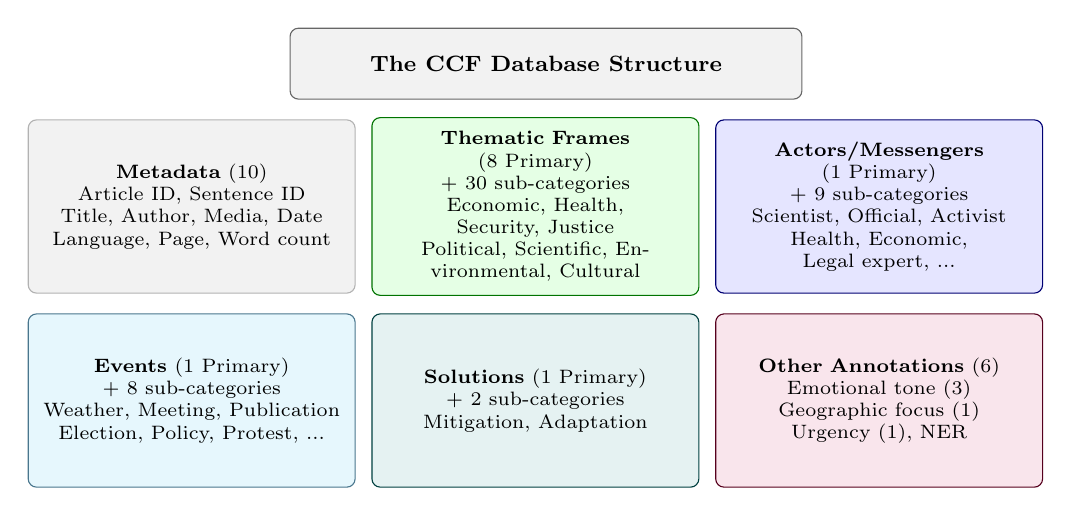
\begin{tikzpicture}[
    node distance=0.25cm and 0.2cm,
    header/.style={rectangle, draw=black!60, rounded corners=3pt, fill=gray!10, minimum width=6.5cm, minimum height=0.9cm, align=center, font=\footnotesize\bfseries},
    group/.style={rectangle, rounded corners=3pt, minimum width=4.0cm, minimum height=2.2cm, align=center, font=\scriptsize, text width=3.8cm, inner sep=5pt},
    group_meta/.style={group, draw=gray!60,   fill=gray!10},
    group_frames/.style={group, draw=green!45!black,  fill=green!10},
    group_actors/.style={group, draw=blue!45!black,   fill=blue!10},
    group_events/.style={group, draw=cyan!50!black,   fill=cyan!10},
    group_solutions/.style={group, draw=teal!50!black, fill=teal!10},
    group_other/.style={group, draw=purple!45!black,  fill=purple!10},
]
\node[header] (head) {The CCF Database Structure};
% Row 1 (three groups)
\node[group_meta, below=of head, xshift=-4.5cm] (meta) {\textbf{Metadata} (10)\\Article ID, Sentence ID\\Title, Author, Media, Date\\Language, Page, Word count};
\node[group_frames, right=of meta] (frames) {\textbf{Thematic Frames} (8 Primary)\\+ 30 sub-categories\\Economic, Health, Security, Justice\\Political, Scientific, Environmental, Cultural};
\node[group_actors, right=of frames] (actors) {\textbf{Actors/Messengers} (1 Primary)\\+ 9 sub-categories\\Scientist, Official, Activist\\Health, Economic, Legal expert, ...};
% Row 2 (three groups)
\node[group_events, below=of meta] (events) {\textbf{Events} (1 Primary)\\+ 8 sub-categories\\Weather, Meeting, Publication\\Election, Policy, Protest, ...};
\node[group_solutions, right=of events] (solutions) {\textbf{Solutions} (1 Primary)\\+ 2 sub-categories\\Mitigation, Adaptation};
\node[group_other, right=of solutions] (other) {\textbf{Other Annotations} (6)\\Emotional tone (3)\\Geographic focus (1)\\Urgency (1), NER};
\end{tikzpicture}
}%
\caption{The CCF database structure organizes 76 columns into logical groups: metadata, primary categories (thematic frames, messengers, events, solutions), their sub-categories, and additional annotations. Sentence text is excluded for copyright compliance; all annotations and metadata are preserved.}
\label{fig:database_structure}
\end{figure}

\section{Technical Validation}

Technical validation of the CCF database and the trained models proceeded in three steps. First, a stratified validation set was constructed in line with established best practices for multi-label classification. Second, a PhD-level expert in climate change politics and policy produced the reference annotations that define the gold standard used for all model evaluation. Third, an independent second annotator replicated the coding following a structured protocol comprising a training phase (sentences 1–600) and a blind coding phase (sentences 601–1000), enabling assessment of inter-coder reliability.

\subsection{Construction of the stratified validation set}

The validation set comprises 1,000 sentences (500 per language) extracted from the fully annotated database using root-inverse probability weighting\footnote{The weighting formula $w_i \propto \sum_j 1/\sqrt{f_j}$ assigns higher sampling probability to sentences containing rare categories, where $f_j$ represents the frequency of category $j$ present in sentence $i$. For example, a sentence annotated with both \textit{Economic Frame} (appearing in 15.4\% of the corpus) and \textit{Loss of Indigenous Practices} (appearing in 0.28\% of the corpus) would receive a weight of approximately $1/\sqrt{0.154} + 1/\sqrt{0.0028} = 2.55 + 18.90 = 21.45$, making it roughly 8 times more likely to be selected than a sentence containing only \textit{Economic Frame}.} combined with strict constraints to ensure statistical validity. Two constraints were applied: first, a minimum threshold of 40 positive examples per category to ensure sufficient statistical power for reliable performance estimation. Without this constraint, rare categories like \textit{Disruption of military operations} (0.00004\% prevalence in the database) would have too few examples to meaningfully assess model accuracy. Second, a 35\% maximum allocation to prevent any single prevalent category from monopolizing the validation set. For instance, without this constraint, \textit{Actors/Messengers Detection} (present in 48.8\% of database sentences) could theoretically dominate the entire sample, leaving insufficient space for other categories.


\begin{figure}[b!]
\centering
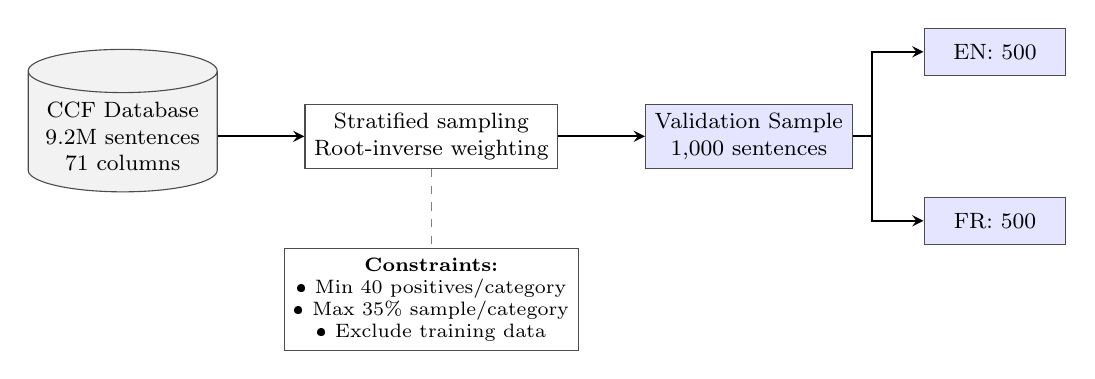
\begin{tikzpicture}[
    box/.style={rectangle, draw=black!70, fill=white, minimum width=2.2cm, minimum height=0.65cm, align=center, font=\footnotesize},
    database/.style={cylinder, draw=black!70, fill=gray!10, minimum width=2.4cm, minimum height=1cm, align=center, shape border rotate=90, aspect=0.25, font=\footnotesize},
    sample/.style={rectangle, draw=black!70, fill=blue!10, minimum width=1.8cm, minimum height=0.6cm, align=center, font=\footnotesize},
    arrow/.style={->, >=stealth, thick},
    node distance=1.1cm
]

% Centered positioning - starting at x=-3.5 for better centering
% Database (left)
\node[database] (db) at (-3.2,0) {\footnotesize CCF Database\\\footnotesize 9.2M sentences\\\footnotesize 71 columns};

% Sampling process (center-left)
\node[box, right=of db] (sampling) {\footnotesize Stratified sampling\\\footnotesize Root-inverse weighting};
\draw[arrow] (db.east) -- (sampling.west);

% Validation sample (center-right)
\node[sample, right=of sampling] (val) {\footnotesize Validation Sample\\\footnotesize 1,000 sentences};
\draw[arrow] (sampling.east) -- (val.west);

% Language split (right) - reduced distances
\node[sample, above right=0.35cm and 0.9cm of val] (en) {\footnotesize EN: 500};
\node[sample, below right=0.35cm and 0.9cm of val] (fr) {\footnotesize FR: 500};
\draw[arrow] (val.east) -- ++(0.25,0) |- (en.west);
\draw[arrow] (val.east) -- ++(0.25,0) |- (fr.west);

% Constraints box (below) - adjusted width
\node[box, below=1cm of sampling, text width=3.5cm, font=\scriptsize] (constraints) {\textbf{Constraints:}\\• Min 40 positives/category\\• Max 35\% sample/category\\• Exclude training data};
\draw[dashed, gray] (sampling.south) -- (constraints.north);

\end{tikzpicture}
\vspace{0.15cm}
\caption{Stratified sampling procedure for final validation. Root-inverse probability weighting ensures balanced representation across all 65 annotation categories.}
\label{fig:validation_sampling}
\end{figure}

\subsection{Expert gold-standard annotation and model performance}

All 1,000 sentences in the validation set were manually annotated by a PhD-level expert specializing in climate change politics and policy. These expert annotations define the gold standard against which all model performance metrics reported in this section are computed.

The validation results demonstrate robust performance across all annotation dimensions, with an overall F1 macro score of 0.866 (0.869 for English, 0.864 for French). As detailed in Table~\ref{tab:detailed_validation_metrics} (Appendix), primary detection categories achieve the highest performance, with \textit{Canadian Context} (F1=0.982) and \textit{Actors/Messengers} (F1=0.961) showing near-perfect classification. Thematic frames maintain strong performance despite their semantic complexity, with \textit{Scientific Frame} (F1=0.890) and \textit{Environmental Frame} (F1=0.871) leading this category. The hierarchical classification strategy proves particularly effective, as evidenced by consistently higher recall scores for detection categories (mean recall=0.891) that trigger conditional sub-category evaluation. Notably, rare categories such as \textit{Disruption of military operations} and \textit{Post-disaster military assistance} show perfect precision despite minimal representation.

To assess temporal stability, stratified validation was conducted across five temporal periods (1980s–2020s) that revealed minimal performance drift ($\Delta$F1 < 1.1\%) despite evolving media discourse patterns (Figure~\ref{fig:temporal_validation}). This temporal consistency validates the models' generalization capacity across the full 46-year corpus span.

\begin{table}[H]
\centering
\caption{Overall validation performance metrics}
\label{tab:final_validation_metrics}
\begin{tabular}{lccc}
\toprule
\textbf{Language} & \textbf{F1 Macro} & \textbf{F1 Micro} & \textbf{F1 Weighted} \\
\midrule
English (EN) & 0.869 & 0.909 & 0.911 \\
French (FR) & 0.864 & 0.902 & 0.905 \\
\midrule
\textbf{Combined (ALL)} & \textbf{0.866} & \textbf{0.905} & \textbf{0.908} \\
\bottomrule
\end{tabular}
\end{table}
\vspace{-0.1em}
\begin{figure}[H]
\centering
\includegraphics[width=0.65\textwidth]{../Results/Outputs/Figures/temporal_f1_evolution.png}
\caption{Temporal validation showing stable F1 macro scores across five time periods. The minimal variation ($\Delta$F1 < 1.1\%) confirms robust model performance without temporal degradation.}
\label{fig:temporal_validation}
\end{figure}

\subsection{Inter-coder assessment of the gold standard}

Inter-coder reliability assessment was completed with a second independent annotator evaluating the same 1,000 randomly selected sentences from the validation set. The protocol followed a structured approach: during the first 600 sentences, the expert annotator provided training to the second coder, explaining category definitions and answering questions without directly intervening in the coding process. This training phase allowed the second coder to progressively learn the annotation framework while maintaining independence in coding decisions. After sentence 600, the annotation process became completely blind, with no communication between coders. The resulting comparison between the second annotator’s labels and the expert gold-standard annotations provides an explicit evaluation of the reliability and reproducibility of the gold standard.

Given that the authors' main interest lies in the level of reliability once the codebook has been learned, the metrics for the blind coding phase (sentences 601–1000) are reported as the primary benchmark. Table~\ref{tab:intercoder_metrics} summarizes the agreement between the second annotator and the expert gold standard across all 65 annotation categories in this phase. These values indicate moderate agreement on Cohen’s $\kappa$ and substantial agreement on Gwet’s AC1, while Krippendorff’s $\alpha$ exceeds the commonly used 0.667 threshold for acceptable reliability. In other words, the gold-standard annotations produced by the expert can be reproduced to a reasonably high degree by an independent trained annotator, even in a setting with 65 multi-label categories and often dense and multi-topic climate discourse.

\begin{table}[b!]
\centering
\caption{Inter-coder reliability metrics for the blind coding phase (sentences 601--1000)}
\label{tab:intercoder_metrics}
\begin{tabular}{lccc}
\toprule
 & Cohen's $\kappa$ & Gwet's AC1 & Krippendorff's $\alpha$ \\
\midrule
Blind coding phase (601--1000) & 0.569 & 0.893 & 0.690 \\
\bottomrule
\end{tabular}
\end{table}

\begin{figure}[H]
\centering
\includegraphics[width=0.65\textwidth]{../Results/Outputs/Figures/intercoder_progression.png}
\caption{Inter-coder reliability progression across 1,000 annotated sentences, computed in successive blocks of 100 sentences.}
\label{fig:intercoder_progression}
\end{figure}

However, several limitations should be kept in mind. The moderate $\kappa$ values reflect the inherent difficulty of climate discourse annotation at the sentence level, where many sentences contain subtle framings and overlapping categories. Chance-corrected indices such as Cohen’s $\kappa$ are also known to be sensitive to category imbalance, which is pronounced in this setting. The substantially higher Gwet’s AC1 suggests that part of the apparent disagreement in $\kappa$ is driven by these prevalence-related paradoxes rather than by systematic confusion between coders. 

To better understand how reliability evolves as the second annotator internalizes the codebook, agreement metrics in successive blocks of 100 sentences were computed. This analysis shows a pattern consistent with a learning curve for a complex codebook: both Cohen’s $\kappa$ and Krippendorff’s $\alpha$ increase over time, with higher values in the later blocks than in the early ones. Figure~\ref{fig:intercoder_progression} illustrates this progression across the 1,000 sentences, with a continuing improvement after the transition to blind coding at sentence 600. The upward trajectory of both indices across the 100-sentence blocks indicates that, once training is complete, the annotation framework can be applied consistently. This reinforces the view that the expert-defined gold standard is reproducible by trained coders.

\begin{figure}[b!]
\centering
\includegraphics[width=\textwidth]{../Results/Outputs/Figures/combined_distributions.png}
\caption{Distribution of annotation categories across the CCF database. The figure shows the average proportion of sentences containing each category for three major annotation groups: \texttt{messenger} (left), \texttt{solution} (center), and \texttt{event} (right). Primary categories represent sentences with any mention of the respective dimension, while subcategories provide more granular classification (see Table \ref{tab:complete_framework} in Appendix for detailed category definitions and variable codes).}
\label{fig:combined_distributions}
\end{figure}

\section{Data Descriptors}

This section demonstrates the analytical capabilities of the CCF database through two complementary perspectives. First, the key distributional characteristics of the annotated data are presented. These baseline distributions provide context for understanding the Canadian climate media landscape and identifying areas for research. Second, four illustrative applications demonstrate how the database's granular annotations can support original analyses: relationships between political actors and climate coverage, regional variations in scientific framing, frame based editorial prioritization, and the network structure of ``epistemic authorities'' (i.e., individuals cited as sources in climate discourse). These examples represent only a fraction of the database's analytical potential; additional statistical modeling incorporating external data sources and advanced computational methods is currently being developed.\footnote{For instance, the authors are developing media cascade detection algorithms that leverage the full cross referenced metadata (journalists, outlets, temporal patterns) to identify information diffusion dynamics across the Canadian media ecosystem. See \url{https://github.com/antoinelemor/CCF-media-cascade-detection} for ongoing work in this direction.}

\subsection{Distribution of Annotation Categories Across the Database}

To understand the composition and characteristics of the CCF database, Figure \ref{fig:combined_distributions} presents the distribution of three key annotation groups across the database (see Table \ref{tab:complete_framework} in Appendix for all variable definitions). The \texttt{messenger} panel reveals that public officials (\texttt{msg\_official}, 33.6\%) and natural scientists (\texttt{msg\_scientist}, 7.8\%) are the most frequently cited actors in climate coverage, while economic experts (\texttt{msg\_economic}, 6.5\%) and cultural figures (\texttt{msg\_cultural}, 3.2\%) receive less attention. This distribution suggests that climate discourse in Canada remains primarily framed through political and scientific lenses. The \texttt{solution} panel demonstrates an overwhelming emphasis on mitigation strategies (\texttt{sol\_mitigation}, 68.7\%) compared to adaptation measures (\texttt{sol\_adaptation}, 3.1\%), indicating that Canadian media coverage focuses predominantly on reducing emissions rather than adaptation. The \texttt{event} panel shows that meetings and conferences (\texttt{evt\_meeting}, 29.0\%) and policy announcements (\texttt{evt\_policy}, 24.9\%) dominate event coverage, while protests (\texttt{evt\_protest}, 0.8\%) and cultural events (\texttt{evt\_cultural}, 1.4\%) receive minimal attention, suggesting an institutional bias in climate reporting.

\begin{figure}[b!]
\centering
\includegraphics[width=\textwidth]{../Results/Outputs/Figures/temporal_frames_evolution.png}
\caption{Temporal evolution of climate frames in Canadian media from 1978 to 2025. Lines represent LOESS-smoothed proportions of sentences containing each frame, with shaded areas indicating 95\% confidence intervals calculated through bootstrap resampling (n=100).}
\label{fig:temporal_evolution}
\end{figure}

The temporal dynamics presented in Figure \ref{fig:temporal_evolution} reveal strong shifts in climate discourse over the last five decades.\footnote{All proportions in this analysis represent the average proportion of sentences per article containing each frame, calculated at the article level before temporal or geographic aggregation.} The most striking pattern is the rise of political framing (\texttt{political\_frame}), which increased from virtually absent in the early 1980s to become the dominant frame by the mid 1990s, stabilizing around 35--40\% of coverage in recent years. This politicization corresponds with a dramatic decline in scientific framing (\texttt{scientific\_frame}), which fell from approximately 40\% in the late 1970s to less than 10\% by 2025. The economic frame (\texttt{economic\_frame}) started around 5\% in the late 1970s, increased progressively to approximately 15\% by the mid 1980s, and has since stabilized at this level. The environmental frame (\texttt{environmental\_frame}), focusing on biodiversity and ecosystem impacts, has maintained a steady but modest presence around 3--5\% of coverage. These patterns indicate a transformation from climate change as primarily a scientific issue, to one dominated by political and economical considerations, with implications for public understanding and policy development.

These distributional analyses demonstrate several key characteristics of the CCF database. First, the comprehensive coverage across all 65 annotation categories validates the framework's ability to capture the multidimensional nature of climate discourse. Second, the temporal and geographic patterns reveal how climate communication has evolved from scientific to political domains. Third, the dominance of institutional actors and events suggests opportunities for diversifying climate narratives to include more grassroots perspectives and adaptation strategies (which may reflect the actual reality of climate policies). Together, these patterns provide researchers with a baseline understanding of Canadian climate discourse that can inform more targeted analyses of specific frames, time periods, or regions.

\subsection{Examples of Analytical Applications}
\label{subsec:analytical_applications}

While the descriptive statistics provide a foundation, the true potential of the CCF database lies in its capacity for accessible analyses, as data are already preprocessed, annotated and validated. Four scientifically grounded applications showcase this potential\endnote{All analysis scripts producing the figures and statistics in this section are available at \url{https://github.com/antoinelemor/CCF-canadian-climate-framing}.}: (1) how political actors shape climate coverage through their relationships with editorial prominence and thematic framing; (2) a cartographic analysis of the geographic polarization of climate science discourse across provinces; (3) how different thematic frames (\texttt{economic\_frame}, \texttt{political\_frame}, \texttt{scientific\_frame}, \texttt{environmental\_frame}, \texttt{justice\_frame}, \texttt{cultural\_frame}) influence newspapers' decisions about front page placement; and (4) the network structure of epistemic authorities, identified through Named Entity Recognition (variable \texttt{ner\_entities}). These are the individuals cited in climate coverage whose cocitation patterns reveal the underlying social architecture of climate communication in Canadian media.


\subsubsection{Political Actors in Climate Coverage}

The CCF database supports targeted analysis of how specific political actors shape climate discourse. Through Named Entity Recognition (\texttt{ner\_entities} variable) applied to all sentences, the database extracts person, organization, and location entities, allowing researchers to identify who speaks about climate change and how they are discussed. Figure~\ref{fig:political_entities} presents the 50 most frequently mentioned persons in 2024 climate coverage.

\begin{figure}[!h]
\vspace*{\fill}
\centering
\includegraphics[width=0.7\textwidth]{../Results/Outputs/Figures/political_debate_entities_front_page_2024.png}
\caption[Most frequently mentioned persons in Canadian climate coverage (2024)]{Top 50 most frequently mentioned persons in Canadian climate coverage (2024). Person entities are extracted from the \texttt{ner\_entities} JSON field (PER category) across all 324,010 sentences. Names are normalized to consolidate variants (e.g., ``Trump'' and ``Donald Trump'' are merged). The dominance of political figures, with Justin Trudeau (11,433 mentions), Donald Trump (9,206), and Pierre Poilievre (6,151) at the top, reflects the politicization of climate discourse in Canadian media.}
\label{fig:political_entities}
\vspace*{0pt}
\end{figure}

The results show that climate coverage in 2024 was dominated by political figures rather than scientists or climate experts. Justin Trudeau leads with 11,433 mentions (5.7\% of all person mentions), followed by Donald Trump (9,206, 4.6\%) and Pierre Poilievre (6,151, 3.1\%). Federal ministers (Steven Guilbeault, Chrystia Freeland), provincial premiers (Danielle Smith, Doug Ford, David Eby), and U.S. political figures (Joe Biden, Kamala Harris) round out the top mentions. This pattern suggests that Canadian media frames climate change primarily through a political lens, with elected officials serving as the dominant voices in climate discourse.

\paragraph{Focused analysis on political leaders.} Beyond identifying who appears in climate coverage, the CCF database allows examination of how specific actors relate to the content of that coverage. Figure~\ref{fig:trudeau_poilievre} examines whether articles mentioning Canada's two major federal party leaders, former Prime Minister Justin Trudeau and Conservative Leader Pierre Poilievre, exhibit different patterns in scientific skepticism framing. Using separate univariate OLS regressions with heteroscedasticity-robust standard errors (HC1), the relationship between leader mention intensity (proportion of article sentences mentioning each leader) and the \texttt{sci\_skepticism} variable is modeled for each leader independently.\endnote{For each leader $\ell \in \{\mathrm{Trudeau}, \mathrm{Poilievre}\}$, we estimate: $\texttt{sci\_skepticism}_{i} = \alpha + \beta_\ell \cdot \mathrm{intensity}_{\ell,i} + \varepsilon_i$, where $\texttt{sci\_skepticism}_{i}$ is the proportion of sentences questioning climate science in article $i$, and $\mathrm{intensity}_{\ell,i}$ is the proportion of sentences mentioning leader $\ell$. The variable \texttt{sci\_skepticism} captures sentences that question the validity, accuracy, or sufficiency of climate science (see Table \ref{tab:complete_framework} in Appendix). Models use HC1 robust standard errors. Leader mentions are identified through pattern matching on the \texttt{ner\_entities} JSON field (PER category). Panel~B compares articles mentioning each leader at least once; Mann-Whitney U tests assess between-group differences. Analysis covers September 10, 2022 (when Poilievre became Conservative leader) to December 31, 2024.}\edef\notetrudeaupoilievre{\theendnote}

\begin{figure}[!t]
\centering
\includegraphics[width=\textwidth]{../Results/Outputs/Figures/trudeau_poilievre_scientific_framing.png}
\caption[Effect of political leader mentions on scientific skepticism]{Effect of political leader mentions on scientific skepticism (\texttt{sci\_skepticism}) from September 2022 to December 2024. Panel~A shows marginal effects from OLS regression with 95\% confidence bands; Panel~B shows aggregate proportions with 95\% bootstrap confidence intervals.\endnotemark[\notetrudeaupoilievre]}
\label{fig:trudeau_poilievre}
\end{figure}

The results reveal a strong asymmetry. Panel A shows that increased mention intensity of Pierre Poilievre is strongly associated with higher scientific skepticism ($\beta=+0.91$, $p<0.001$), while Justin Trudeau shows a weaker but still significant association ($\beta=+0.29$, $p<0.001$). The effect of Poilievre on skepticism is approximately three times stronger than that of Trudeau. Panel B confirms these patterns at the aggregate level: articles mentioning Poilievre contain significantly higher proportions of scientific skepticism classified sentences compared to articles mentioning Trudeau. Based on 25,351 articles from the period when Poilievre served as Conservative leader, 4,115 articles (16.2\%) mention Trudeau and 1,834 (7.2\%) mention Poilievre, with 1,331 (5.3\%) mentioning both leaders. These findings suggest that media coverage associating Poilievre with climate issues more frequently employs frames that question scientific consensus, potentially reflecting both the leader's public stance on climate policy and editorial choices about how to contextualize his positions. This type of actor frame association analysis, impossible with traditional content analysis methods, becomes straightforward with the CCF database's preannotated structure.

\subsubsection{Geographic Polarization of Climate Science Discourse}

The CCF database also supports detailed geographic analysis of how climate science is discussed across Canadian provinces. Figure \ref{fig:science_acceptance} reveals regional patterns in scientific skepticism. The analysis focuses on the \texttt{sci\_skepticism} subcategory (see Table \ref{tab:complete_framework} in Appendix), which captures sentences that question the validity, accuracy, or sufficiency of climate science, including challenges to climate models, dismissals of scientific evidence, or expressions of doubt about the scientific consensus.

Panel~A reveals geographic variation in the prevalence of scientific skepticism across provinces. Among sentences with scientific content, the proportion expressing skepticism varies notably across regions. Western provinces show distinct patterns compared to Eastern Canada. The Prairie provinces (Saskatchewan, Alberta) along with British Columbia display varying rates of skepticism framing, while Quebec and the Atlantic provinces show different levels.

Panels~B and~C extend this geographic analysis by examining how political leader mentions correlate with scientific skepticism framing at the provincial level, using separate univariate OLS regressions for each province-leader combination.\endnote{For each province $p$ and leader $\ell \in \{\mathrm{Trudeau}, \mathrm{Poilievre}\}$, we estimate: $\texttt{sci\_skepticism}_{i} = \alpha_p + \beta_{p,\ell} \cdot \mathrm{intensity}_{i,\ell} + \varepsilon_i$, where $\mathrm{intensity}_{i,\ell}$ is the proportion of article sentences mentioning leader $\ell$. The variable \texttt{sci\_skepticism} captures sentences that question the validity, accuracy, or sufficiency of climate science (see Table \ref{tab:complete_framework} in Appendix). Coefficients $\beta$ represent the change in skepticism framing per unit increase in leader mention intensity. Analysis covers September 10, 2022 (when Poilievre became Conservative leader) to December 31, 2024. Only provinces with $\geq$50 articles and $\geq$10 articles mentioning the leader are shown. Significance: *** $p<0.001$, ** $p<0.01$, * $p<0.05$. Hatched areas indicate insufficient data.}\edef\notegeographic{\theendnote} The contrast between leaders is striking: Trudeau mentions show a significant positive association with skepticism in Ontario ($\beta=+0.77$, $p<0.001$) and Yukon ($\beta=+0.77$, $p<0.05$), with no significant effects in other provinces. In contrast, Poilievre mentions are significantly associated with increased skepticism across multiple provinces: Quebec ($\beta=+1.53$, $p<0.001$), British Columbia ($\beta=+1.33$, $p<0.001$), Saskatchewan ($\beta=+1.31$, $p<0.001$), and Alberta ($\beta=+1.19$, $p<0.001$). This asymmetry suggests that coverage mentioning the Conservative leader is more systematically linked to skeptical framings of climate science, particularly in Western provinces and Quebec.

\begin{figure}[t]
\centering
\includegraphics[width=\textwidth]{../Results/Outputs/Figures/science_acceptance_maps.png}
\caption[Geographic patterns of scientific skepticism and political leader effects]{Geographic patterns of scientific skepticism (\texttt{sci\_skepticism}) in Canadian climate coverage. Panel~A shows the proportion of scientific skepticism among scientific sentences (all years). Panels~B and~C show the effect of leader mention intensity on scientific skepticism framing (September 2022--December 2024), estimated via OLS regression with robust standard errors.\endnotemark[\notegeographic]}
\label{fig:science_acceptance}
\end{figure}

\begin{figure}[htbp]
\centering
\includegraphics[width=\textwidth]{../Results/Outputs/Figures/frames_front_page_probability.png}
\caption[Effect of frame intensity on front page placement]{Effect of frame intensity on front page placement probability. Panel~A shows predicted probabilities from logistic regression as frame intensity increases; Panel~B shows regression coefficients with 95\% confidence intervals.\endnote{For each thematic frame $f \in \{$\texttt{economic\_frame}, \texttt{political\_frame}, \texttt{scientific\_frame}, \texttt{environmental\_frame}, \texttt{justice\_frame}, \texttt{health\_frame}, \texttt{security\_frame}, \texttt{cultural\_frame}$\}$, we estimate a separate univariate logistic regression model: $\mathrm{logit}(P(\mathrm{FrontPage})) = \alpha_f + \beta_f \cdot \mathrm{intensity}_f$, where $\mathrm{intensity}_f$ is the proportion of article sentences containing frame $f$. Coefficients $\beta_f$ represent the change in log-odds of front page placement per unit increase in frame intensity. Predicted probabilities in Panel~A are computed as $\hat{P} = 1/(1+e^{-(\hat{\alpha}_f+\hat{\beta}_f \cdot x)})$. Confidence bands use the delta method. All models fit on 266,224 articles (22,884 front page, baseline rate: 8.6\%). All coefficients significant at $p<0.001$.}}
\label{fig:frames_front_page}
\end{figure}
\edef\noteframes{\theendnote}

\subsubsection{Frame Based Editorial Prioritization}

The CCF database can reveal patterns in how different climate frames influence editorial decisions about story prominence. Rather than simply comparing frame presence, this analysis models the relationship between frame intensity (the proportion of article sentences containing each frame) and front page placement probability using separate univariate logistic regressions for each frame.\endnotemark[\noteframes]

Figure~\ref{fig:frames_front_page} shows a striking pattern in editorial prioritization. Panel~A displays predicted front page probability curves as frame intensity increases from 0\% to 100\% of article content. Only two frames show positive associations with editorial prominence: \texttt{economic\_frame} ($\beta=+0.98$, $p<0.001$) and \texttt{political\_frame} ($\beta=+0.18$, $p<0.001$). As the proportion of economic framing increases in an article, front page probability rises substantially, from the 8.6\% baseline to over 20\% for articles dominated by economic content. All other frames exhibit significant negative associations: \texttt{security\_frame} ($\beta=-2.80$), \texttt{health\_frame} ($\beta=-2.07$), \texttt{environmental\_frame} ($\beta=-1.27$), \texttt{scientific\_frame} ($\beta=-0.96$), \texttt{justice\_frame} ($\beta=-0.79$), and \texttt{cultural\_frame} ($\beta=-0.32$), all $p<0.001$. Panel~B visualizes these effect sizes, with positive coefficients (right of zero) indicating frames that increase editorial prominence. These findings suggest that Canadian newspapers systematically privilege economic and political framings of climate change in their most prominent coverage, while scientific, environmental, and health perspectives receive lower editorial priority. This pattern has potential implications for public understanding of climate change as primarily an economic or political issue rather than an environmental or scientific one.

\subsubsection{Network Structure of Epistemic Authorities}

\begin{figure}[t!]
\centering
\includegraphics[width=0.7\textwidth]{../Results/Outputs/Figures/network.pdf}
\caption{Cocitation network of epistemic authorities in Canadian climate media discourse (year=2024). Node size represents degree centrality, edge thickness indicates cocitation frequency, and colors denote community detection clusters. The network reveals a hierarchical structure with political figures at the core (Trudeau: degree centrality 0.899, Poilievre: 0.818, Trump: 0.667) and six interconnected communities: federal Canadian politics (community 3), US/international figures (community 1), Ontario (community 6), Québec (community 0), British Columbia (community 2), and historical political figures (community 5). Activist Greta Thunberg (community 4) appears isolated with no cocitation links to other top authorities.}
\label{fig:network}
\end{figure}

The CCF database also supports network analysis of ``epistemic authorities,'' the individuals cited in climate discourse. Using Named Entity Recognition (\texttt{ner\_entities}), this approach extracts all persons mentioned in climate coverage and maps their cocitation patterns (i.e., cooccurrence within the same article), thus revealing the underlying social structure of climate communication. Further analyses can filter by messenger type using the \texttt{messenger} category and its subcategories (\texttt{msg\_scientist}, \texttt{msg\_official}, \texttt{msg\_activist}, etc.) to focus specifically on quoted sources. 


Figure \ref{fig:network} presents a cocitation network of persons mentioned in 2024 climate coverage.\endnote{The network analysis proceeds in four stages: (1) person entities are extracted from the \texttt{ner\_entities} field across all 2024 sentences; (2) names are normalized using automated resolution and manual verification for high-profile figures; (3) persons are aggregated at the article level; (4) cocitation networks are constructed where an edge connects two persons mentioned in the same article. For visualization clarity, only the top 100 persons by mention frequency are shown, with edges requiring at least 3 cocitations. For more details, see \url{https://github.com/antoinelemor/CCF-canadian-climate-framing}.} The 2024 network topology shows a highly centralized structure dominated by political figures. Justin Trudeau (1,485 citations), Pierre Poilievre (933 citations), and Donald Trump (793 citations) form the central core, while scientific authorities occupy peripheral positions. The network exhibits high clustering (coefficient = 0.686), with seven detected communities: a dominant federal Canadian cluster (Trudeau, Poilievre, Guilbeault, Freeland, Wilkinson, Singh), a US/international cluster (Trump, Biden, Harris, Putin, Musk), provincial clusters for Ontario (Ford, Chow, Crombie), Québec (Legault, Charette, Plante), and British Columbia (Eby, Rustad, Furstenau), a historical figures cluster (Mulroney, Reagan, Thatcher, Pierre Trudeau, Chrétien), and an isolated community containing only Greta Thunberg, the sole activist with no cocitation links to other top 100 authorities.

The dominance of political over scientific authorities is clear: 19 of the top 20 authorities are politicians, Elon Musk (rank 18) is the only nongovernmental figure (at least at the time). This pattern reveals that Canadian media frames climate change primarily through political rather than scientific lenses. Combined with the earlier finding that articles mentioning Poilievre are significantly more associated with scientific skepticism framing (\texttt{sci\_skepticism}), this network structure suggests that expertise itself becomes politicized in climate communication. The high clustering coefficient indicates that media coverage reinforces topical silos rather than fostering dialogue across domains, with authorities cited within specialized communities that rarely intersect. 

\section{Bridging Scale and Granularity in Climate Discourse Analysis}

The Canadian Climate Framing (CCF) database establishes a new paradigm for climate communication research by combining scale, granularity, and machine learning within a single infrastructure. Transforming 266,271 articles across 46 years into 9.2 million analysis ready sentences with 65 validated annotations variables and NER, the CCF supports new analyses that were impossible before. Its four phase architecture and reproducible annotation framework address longstanding methodological limitations and can be adapted to examine contexts beyond Canada, supporting comparative work on how media agendas interact across different national settings. 

With an overall F1 score of 0.866, and strong performance even for underrepresented categories, the database shows that computational methods can capture the semantic complexity of climate discourse with sufficient accuracy for rigorous research. Although the analytical categories and newspaper selection inevitably involve interpretive choices and remain open to refinement, the CCF database nonetheless represents a significant advance. 

Beyond its technical contribution, the CCF provides a dynamic research infrastructure: it will be regularly updated to incorporate the latest coverage, and scholars can experiment with its annotation categories to explore frame combinations, messenger strategies, emotional tone, or spatiotemporal patterns. Ultimately, the CCF database helps to strengthen climate communication as an evidence-informed social science and provides a foundation for developing more effective communication strategies.

\section{Acknowledgments}

The authors thank Richard Nadeau for his valuable input throughout the development of this project. The authors also acknowledge the research assistance of Maëlle Rouyer. Earlier versions of this paper were presented at the annual meetings of the Canadian Political Science Association, the Prairie Political Science Association, and the American Political Science Association, as well as at the University of Montreal. The authors wish to acknowledge the anonymous reviewers and editor for their feedback throughout the development of this paper.

\section{Author Contributions}

Blabla

\section{Funding}

Funding for this research was provided by the Fonds de recherche du Québec [FRQ Grant number \href{https://doi.org/10.69777/337081}{337081}].

\newpage
\printendnotes



\appendix
\setcounter{table}{0}  % Reset table counter for appendix
\renewcommand{\thetable}{A\arabic{table}}  % Prefix appendix tables with 'A'
\renewcommand\theHtable{Appendix.\thetable}  % Fix hyperref links for appendix tables

% Appendix A: Literature Review
\landscape
\section{Appendix A: Previous Studies on Canadian Climate Media Coverage}
\label{sec:appendix_literature}

{\footnotesize
\begin{longtable}{p{5cm}p{6cm}p{4cm}p{3cm}p{3.5cm}}
\caption{Summary of previous studies analyzing climate change coverage in Canadian newspapers}
\label{tab:literature_review}
\\
\toprule
\textbf{Study} & \textbf{Newspaper(s)} & \textbf{Scope} & \textbf{Language} & \textbf{Time Period} \\
\midrule
\endfirsthead
\multicolumn{5}{c}{\tablename\ \thetable\ -- \textit{Continued from previous page}} \\
\toprule
\textbf{Study} & \textbf{Newspaper(s)} & \textbf{Scope} & \textbf{Language} & \textbf{Time Period} \\
\midrule
\endhead
\midrule
\multicolumn{5}{r}{\textit{Continued on next page}} \\
\endfoot
\bottomrule
\endlastfoot

\textcite{good_framing_2008} & The Globe and Mail & National & English & 2007 \\
& The National Post & National & English & \\
& The Toronto Star & National & English & \\
& The Calgary Herald & Regional & English & \\
& The Edmonton Journal & Regional & English & \\
& The Chronicle Herald & Regional & English & \\
& The Montreal Gazette & Regional & English & \\
& The Charlottetown Guardian & Regional & English & \\
& Halifax Daily News & Regional & English & \\
& The Ottawa Citizen & Regional & English & \\
& The Star Phoenix & Regional & English & \\
& The Telegram & Regional & English & \\
& The Times Colonist & Regional & English & \\
& The Vancouver Sun & Regional & English & \\
& The Winnipeg Sun & Regional & English & \\
& Yukon News & Regional & English & \\
\midrule
\textcite{rowe_comparing_2011} & The Globe and Mail & National & English & 2007--2008 \\
& The Toronto Star & National & English & \\
& The Calgary Herald & Regional & English & \\
& The Toronto Sun & Regional & English & \\
& The Montreal Gazette & Regional & English & \\
& The Ottawa Citizen & Regional & English & \\
\midrule
\textcite{young_representations_2011} & The Globe and Mail & National & English & 1988--2008 \\
& The National Post & National & English & \\
\midrule
\textcite{anne_difrancesco_seeing_2011} & The Globe and Mail & National & English & 2008 \\
& The National Post & National & English & \\
\midrule
\textcite{ahchong_anthropogenic_2012} & The Globe and Mail & National & English & 1988--2007 \\
& The Toronto Star & National & English & \\
\midrule
\textcite{stoddart_canadian_2015} & The Globe and Mail & National & English & 1999--2010 \\
& The National Post & National & English & \\
\midrule
\textcite{ford_coverage_2015} & The Globe and Mail & National & English & 1993--2013 \\
& The Toronto Star & National & English & \\
\midrule
\textcite{stoddart_endangered_2016} & The Globe and Mail & National & English & 2006--2010 \\
& The National Post & National & English & \\
\midrule
\textcite{stoddart_media_2017} & The Globe and Mail & National & English & 1997--2010 \\
& The National Post & National & English & \\
\midrule
\textcite{barkemeyer_media_2017} & The Globe and Mail & National & English & 2008 \\
& The National Post & National & English & \\
& The Toronto Star & National & English & \\
& The Vancouver Sun & Regional & English & \\
& The Toronto Sun & Regional & English & \\
\midrule
\textcite{king_how_2019} & The Globe and Mail & National & English & 2005--2015 \\
& The National Post & National & English & \\
& The Toronto Star & National & English & \\
& The Calgary Herald & Regional & English & \\
& The Chronicle Herald & Regional & English & \\
& The Vancouver Sun & Regional & English & \\
& The Whitehorse Daily Star & Regional & English & \\
& Journal de Montréal & Regional & French & \\
\midrule
\textcite{pillod_reframing_2021} & The Globe and Mail & National & English & 2008--2020 \\
\midrule
\cite{brandt_news_2021} & The Toronto Star & National & English & 2015--2018 \\
& The Calgary Herald & Regional & English & \\
& The Vancouver Sun & Regional & English & \\
& The Chronicle Herald & Regional & English & \\
& The Winnipeg Free Press & Regional & English & \\
& Times and Transcript & Regional & English & \\
\midrule
\textcite{hase_climate_2021} & The Globe and Mail & National & English & 2006--2018 \\
& The Toronto Star & National & English & \\
\midrule
\textcite{sachdeva_themes_2022} & n/a & n/a & English & 1986--2016 \\
\midrule
\textcite{stoddart_what_2023} & The Globe and Mail & National & English & 2015--2020 \\
& The National Post & National & English & \\
& The Telegraph & Regional & English & \\
& The Telegram & Regional & English & \\
& The Chronicle Herald & Regional & English & \\
& The Guardian & Regional & English & \\
\midrule
\textcite{chen_how_2023} & n/a & n/a & English & 2018--2021 \\
\bottomrule
\end{longtable}
}

\vspace{0.5em}
\noindent\footnotesize
Note: This table summarizes the newspaper sources, geographic scope, language, and time periods covered by previous studies on climate change media coverage in Canada. Most studies focus exclusively on English-language national newspapers, particularly The Globe and Mail and The National Post.
\endlandscape

% Appendix B: Complete Framework and Performance Metrics
\setcounter{table}{0}  % Reset table counter for appendix B
\renewcommand{\thetable}{B\arabic{table}}  % Prefix appendix B tables with 'B'
\renewcommand\theHtable{AppendixB.\thetable}  % Fix hyperref links for appendix B tables

\landscape
\section{Appendix B: Complete Framework and Performance Metrics}
\label{sec:appendix}
{\footnotesize
\phantomsection
\begin{longtable}{p{0.5cm}p{4.5cm}p{2.8cm}p{13.5cm}}
\caption{Complete CCF annotation framework: All 65 categories with operational definitions and database codes}
\label{tab:complete_framework}
 \\
\toprule
\textbf{\#} & \textbf{Category} & \textbf{Code} & \textbf{Description} \\
\midrule
\endfirsthead
\multicolumn{4}{c}{\tablename\ \thetable\ -- \textit{Continued from previous page}} \\
\toprule
\textbf{\#} & \textbf{Category} & \textbf{Code} & \textbf{Description} \\
\midrule
\endhead
\midrule
\multicolumn{4}{r}{\textit{Continued on next page}} \\
\endfoot
\bottomrule
\endlastfoot

\multicolumn{4}{l}{\cellcolor{gray!10}\textbf{THEMATIC FRAMES}} \\
\midrule
\rowcolor{gray!8}
\multicolumn{4}{l}{\textit{Economic Frame}} \\
\midrule
1 & \textbf{Economic Frame\newline (Primary Category)} & \texttt{economic\_frame} & If the sentence refers to climate change as an economic issue, including its negative or positive impacts on the economy, the financial costs or benefits of climate action, or the carbon footprint of the economic or industrial sector. This label captures any framing of climate change in economic terms, such as effects on jobs, markets, industries, or public and private finances. \\
\cmidrule(lr){1-4}
2 & Negative impacts of climate change on the economy & \texttt{eco\_neg\_impact} & If the sentence refers to the negative effects of climate change on the economy, such as damage to infrastructure, loss of agricultural productivity, disruptions to trade, increased costs for businesses, or economic decline in sectors vulnerable to climate shifts. This includes any economic losses directly resulting from changing climate conditions. \\
3 & Positive impacts of climate change on the economy & \texttt{eco\_pos\_impact} & If the sentence refers to the positive effects of climate change on the economy, such as new agricultural opportunities, the opening of new trade routes, or the potential for economic growth in sectors adapting to climate shifts. This includes any economic gains directly resulting from changing climate conditions. \\
4 & Economic disadvantages of climate action & \texttt{eco\_cost} & If the sentence refers to the negative economic impacts caused by climate policies or climate action, such as costs associated with transitioning to green energy, investments in climate adaptation, debt incurred from financing climate action, or short-term job losses in fossil fuel industries. This category captures financial burdens and challenges linked to climate action or policy. \\
5 & Economic benefits of climate action & \texttt{eco\_benefit} & If the sentence refers to the positive economic impacts resulting from climate policies or climate action, such as job creation in renewable energy sectors, investments in green technologies, economic growth driven by sustainability initiatives, or cost savings from energy efficiency. This category captures financial gains and opportunities linked to climate action or policy. \\
6 & Carbon footprint of the economic sector & \texttt{eco\_footprint} & If the sentence refers to the environmental or carbon footprint of the economic or industrial sectors, including emissions and resource use related to manufacturing, transportation, energy production, mining, agriculture, and other commercial or industrial activities. This label covers the ecological impact generated by economic and industrial processes, not the effects of climate change on these sectors. \\
\midrule
\rowcolor{gray!8}
\multicolumn{4}{l}{\textit{Health Frame}} \\
\midrule
7 & \textbf{Health Frame\newline (Primary Category)} & \texttt{health\_frame} & If the sentence refers to climate change as a public health issue, including its negative or positive impacts on physical or mental health, the health co-benefits of climate action (e.g., cleaner air, active transportation), or the carbon footprint of the health sector. This label captures any framing of climate change in relation to health outcomes, healthcare systems, or health-related consequences and solutions. \\
\cmidrule(lr){1-4}
8 & Negative impacts of climate change on health & \texttt{health\_neg\_impact} & If the sentence refers to the negative effects of climate change on human health, such as increased risks of infectious diseases (e.g., malaria, dengue), respiratory and cardiovascular illnesses due to air pollution and heat exposure, heat-related illnesses (e.g., heatstroke), and mental health disorders (e.g., anxiety, depression) linked to environmental changes. \\
9 & Health co-benefits of climate action & \texttt{health\_cobenefit} & If the sentence refers to health benefits resulting from climate policies or actions, such as improved air quality, better nutrition, reduced respiratory or cardiovascular diseases, fewer premature deaths, and other positive health outcomes linked to climate mitigation and adaptation efforts. \\
\midrule
\rowcolor{gray!8}
\multicolumn{4}{l}{\textit{Security Frame}} \\
\midrule
10 & \textbf{Security Frame\newline (Primary Category)} & \texttt{security\_frame} & If the sentence refers to the effects of climate change on security, such as violent conflict driven by resource scarcity, an influx of climate refugees, disruption of military operations, or the carbon footprint of the defense sector. This category includes broader security challenges arising from climate change, including geopolitical tensions or the strategic responses to climate impacts. \\
\cmidrule(lr){1-4}
11 & Presence of climate refugees & \texttt{security\_refugees} & If the sentence refers to the displacement of populations or the presence of climate refugees as a result of a natural disaster, environmental degradation, or climate change impact. This category captures the movement of people fleeing climate-related disasters. \\
12 & Conflict & \texttt{security\_conflict} & If the sentence refers to the emergence or intensification of conflicts over natural resource exploitation due to climate change, such as disputes over water, land, or energy resources exacerbated by shifting climate patterns. This includes conflicts arising from scarcity or competition for increasingly stressed resources. \\
13 & \textit{Post-disaster military assistance}* & \texttt{security\_military} & If the sentence refers to the deployment of military forces as reinforcement after a natural disaster, such as wildfires, floods, or other extreme events. This includes military support in disaster response and recovery, like providing humanitarian aid or maintaining order during a crisis. \\
14 & \textit{Disruption of military operations}* & \texttt{security\_disruption} & If the sentence refers to the disruption of military operations due to a natural disaster affecting a military base or facilities. This includes cases where climate-induced events damage or disrupt military infrastructure, affecting defense readiness or response capabilities. \\
\midrule
\rowcolor{gray!8}
\multicolumn{4}{l}{\textit{Justice Frame}} \\
\midrule
15 & \textbf{Justice Frame\newline (Primary Category)} & \texttt{justice\_frame} & If the sentence frames climate change as a justice or moral issue, including references to who benefits or loses from climate action, differentiated responsibilities across countries or groups, unequal impacts of climate change, disparities in access to mitigation or adaptation measures, or concerns about intergenerational justice. This label captures ethical, equity-based, or fairness-oriented dimensions of climate discourse. \\
\cmidrule(lr){1-4}
16 & Winners and losers of climate action & \texttt{justice\_winners} & If the sentence refers to how climate policies or actions create winners and losers, by benefiting certain groups (e.g., vulnerable populations, Indigenous communities, developing countries) while disadvantaging others (e.g., fossil fuel workers, carbon-intensive industries, or developed nations facing steeper transitions). This label focuses on distributional outcomes of climate policy. \\
17 & Differentiated responsibility & \texttt{justice\_responsibility} & If the sentence refers to the unequal responsibility for causing climate change, especially in reference to the principle of common but differentiated responsibilities. This includes statements emphasizing that developed countries, multinational corporations, or high-emitting individuals have historically contributed more to global warming and should therefore bear a greater share of the mitigation burden. \\
18 & Unequal vulnerability to climate change & \texttt{justice\_vulnerability} & If the sentence highlights how different populations are unequally affected by the impacts of climate change, due to geographic, social, or economic vulnerabilities. This includes references to marginalized groups such as women, seniors, racialized populations, people in developing countries, or those living in high-risk zones (e.g., coastal or arid regions). This label focuses on impacts, not responsibility or capacity. \\
19 & Unequal access to climate action & \texttt{justice\_access} & If the sentence refers to unequal capacity to act on climate change, emphasizing that countries, companies, or individuals do not have equal financial, technical, or institutional means to take climate action. For example, small businesses may struggle to decarbonize compared to multinational firms, and low-income households may not afford sustainable alternatives. This label reflects inequality in ability to act, not impacts or blame. \\
20 & Intergenerational justice & \texttt{justice\_intergen} & If the sentence refers to intergenerational justice, meaning that current decisions and actions should not compromise the rights or well-being of future generations. Do not apply this label to sentences that merely mention age differences or generational groups (e.g., ``young people are protesting'') unless the statement clearly relates to moral responsibility across generations or the long-term consequences of climate inaction. \\
\midrule
\rowcolor{gray!8}
\multicolumn{4}{l}{\textit{Political Frame}} \\
\midrule
21 & \textbf{Political Frame\newline (Primary Category)} & \texttt{political\_frame} & If the sentence frames climate change as a political issue, including references to policy adoption or implementation, political debates or controversies, political positioning by parties or leaders on climate issues, and public opinion data related to climate change. This label captures the role of governance, decision-making, and political dynamics in climate discourse. \\
\cmidrule(lr){1-4}
22 & Policy action & \texttt{pol\_action} & If the sentence refers to the formal approval, adoption, or enactment of a policy, plan, or strategy by a government at the local, provincial, national, or international level. This includes the passing of new legislation, regulations, government programs, or official commitments related to climate or environmental issues (e.g., approval of a carbon pricing law, ratification of a renewable energy policy, adoption of a climate action framework). \\
23 & Political debate & \texttt{pol\_debate} & If the sentence refers to a political debate or discussion about climate change, particularly focusing on the differing views or disagreements on climate policies, the effectiveness of past actions, or the responsibility of different levels of government (e.g., federal vs. provincial). This includes disagreements about specific climate initiatives, such as proposed or enacted policies, laws, or funding allocations. \\
24 & Political positioning & \texttt{pol\_position} & If the sentence refers to the explicit stance or position of a politician or political party on climate change or climate-related policies. This includes statements where a political figure or party expresses their support or opposition to specific climate actions (e.g., carbon taxes, energy transitions, or climate mitigation strategies), or when they make electoral promises regarding climate policies. \\
25 & Public opinion data & \texttt{pol\_opinion} & If the sentence refers to data, surveys, polls, or studies measuring public opinion, attitudes, beliefs, or perceptions related to climate change, environmental policies, or climate action. This label captures quantitative or qualitative information on how the public views climate issues. \\
\midrule
\rowcolor{gray!8}
\multicolumn{4}{l}{\textit{Scientific Frame}} \\
\midrule
26 & \textbf{Scientific Frame\newline (Primary Category)} & \texttt{scientific\_frame} & If the sentence frames climate change as a scientific issue, including references to scientific research, discoveries, explanations, or assessments of climate change. This includes mentions of scientific consensus or controversy, as well as expressions of uncertainty or certainty in climate science. This label captures the role of scientific knowledge and expertise in understanding and communicating climate change. \\
\cmidrule(lr){1-4}
27 & Scientific debate & \texttt{sci\_debate} & If the sentence refers to a past or ongoing debate or disagreement within the scientific community about aspects of climate science or climate-related technologies. This includes contested interpretations of data, disputes about methodologies, or ethical debates surrounding proposed scientific or technological solutions such as geoengineering. It does not include general questioning of climate science or statements that challenge the validity or sufficiency of climate evidence. \\
28 & Popularisation or scientific discovery & \texttt{sci\_discovery} & If the sentence explains or describes climate science mostly grounded in the natural sciences---such as chemistry, physics, or biology---or presents scientific or technological discoveries related to climate change. This includes explanations of mechanisms (e.g., the greenhouse effect, climate feedbacks), climate modeling, or innovations such as carbon capture. It does not apply to statements that merely describe environmental conditions or trends without explaining an underlying scientific process. \\
29 & Questioning of climate science & \texttt{sci\_skepticism} & If the sentence questions the validity, accuracy, or sufficiency of climate science. This includes claims that climate projections are flawed, evidence is lacking, or conclusions are exaggerated. It only applies when science is being challenged or delegitimized, not when scientists acknowledge limitations, complexity, or areas of ongoing research. \\
30 & Defense of climate science & \texttt{sci\_defense} & If the sentence defends the robustness or credibility of climate science in response to skepticism or denial. This includes assertions that reinforce the scientific consensus, affirm the validity of climate models, or rebut claims that climate science is incorrect or misleading. It only applies when climate science is defended, not when it is neutrally presented. \\
\midrule
\rowcolor{gray!8}
\multicolumn{4}{l}{\textit{Environmental Frame}} \\
\midrule
31 & \textbf{Environmental Frame\newline (Primary Category)} & \texttt{environmental\_frame} & If the sentence frames climate change as an environmental issue, including references to the degradation or disappearance of natural habitats, loss of biodiversity, and negative impacts on fauna and flora. This label captures ecological consequences of climate change and emphasizes the relationship between climate disruption and the natural environment. \\
\cmidrule(lr){1-4}
32 & Loss of natural environments & \texttt{env\_habitat} & If the sentence refers to the long-term or irreversible disappearance or degradation of natural environments due to climate change. This includes situations where ecosystems or environmental features (e.g., glaciers, coral reefs) are predicted or expected to permanently disappear or significantly decline as a result of climate impacts, indicating that they will not recover. It does not apply to short-term, isolated, or recoverable events, such as one-time disasters (e.g., a single wildfire or a temporary drought) that might affect natural environments but do not necessarily imply permanent loss. \\
33 & Loss of fauna and flora & \texttt{env\_species} & If the sentence refers to the negative impacts of climate change on animal and plant species, including changes in habitat, shifts in migration or breeding patterns, increased mortality, loss of biodiversity, or threats to species survival. This label covers both temporary and ongoing effects on fauna and flora caused by climate change. \\
\midrule
\rowcolor{gray!8}
\multicolumn{4}{l}{\textit{Cultural Frame}} \\
\midrule
34 & \textbf{Cultural Frame\newline (Primary Category)} & \texttt{cultural\_frame} & If the sentence frames climate change as a cultural issue, including cultural depictions of climate change through art, literature, music, or film; challenges to hosting artistic or sports events due to climate impacts; the loss or disruption of Indigenous cultural practices; or the carbon footprint of the cultural and creative sectors. This label captures how climate change affects and is expressed through cultural life and identities. \\
\cmidrule(lr){1-4}
35 & Artistic representation & \texttt{cult\_art} & If the sentence refers to cultural representations of climate change in various forms such as art, literature, music, film, documentaries, theater, or other creative expressions. This label captures how climate change is portrayed, interpreted, or communicated through cultural and artistic mediums. \\
36 & Difficulty to host cultural or sports events & \texttt{cult\_event\_impact} & If the sentence refers to how climate change disrupts or challenges the organization of artistic, cultural, or sports events, such as cancelled festivals, concerts, or competitions due to extreme weather (e.g., storms, heatwaves, wildfires, or lack of snow for winter sports). This label captures climate-related obstacles to event planning or continuity. \\
37 & Loss of indigenous practices & \texttt{cult\_indigenous} & If the sentence refers to the erosion or disruption of traditional cultural practices among Indigenous communities due to climate change, such as changes in animal migration, plant cycles, or land access that affect food systems, ceremonies, or knowledge transmission. This label emphasizes climate-driven impacts on Indigenous cultural continuity. \\
38 & Carbon footprint of the cultural and sports sectors & \texttt{cult\_footprint} & If the sentence refers to the environmental or carbon footprint of the cultural, artistic, or sports sectors, including the emissions and resource use associated with activities such as touring, international travel, energy-intensive venues, unsustainable stage or set production, or event-related waste. This label covers the ecological impact of producing and hosting cultural or sports events, not the impacts of climate on those events. \\
\midrule
\multicolumn{4}{l}{\cellcolor{gray!10}\textbf{PRIMARY CATEGORIES}} \\
\midrule
\rowcolor{gray!8}
\multicolumn{4}{l}{\textit{Actors/Messengers}} \\
\midrule
39 & \textbf{Presence of Messengers\newline (Primary Category)} & \texttt{messenger} & If the sentence includes mentions or quotes of persons or organizations by journalists, whether through direct quotations or indirect references. This label captures the presence of sources, experts, officials, activists, or other actors cited or named within the text. A single individual or organization may be associated with multiple types of expertise or roles (e.g., a doctor would fall both under Health expert and Natural scientist). \\
\cmidrule(lr){1-4}
40 & Health expert & \texttt{msg\_health} & If the quoted or reported statement comes from a person or organization with medical or health-related recognized expertise. This includes individuals working in the fields of medicine, public health, healthcare administration, or biomedical research, whether in a professional, academic, or governmental capacity (e.g., professor of public health, doctor, nurse, family physician, public health officer, WHO representative, Red Cross medical coordinator, Doctors without Borders spokesperson, Canadian Medical Association representative, certified health consultants, minister of Health). \\
41 & Economic expert & \texttt{msg\_economic} & If the quoted or reported statement comes from a person or organization with economic or financial recognized expertise. This includes individuals working in the fields of economics, finance, business, or economic policy, whether in a professional, academic, private sector, or governmental capacity (e.g., economist, finance minister, central bank official, business executive, investment analyst, professor of economics, representative of a chamber of commerce, World Bank or IMF spokesperson, economic think tank expert, labour market analyst). \\
42 & Security expert & \texttt{msg\_security} & If the quoted or reported statement comes from a person or organization with recognized expertise in security or defence matters. This includes individuals with academic, professional, or operational experience in military, national security, intelligence, or strategic affairs (e.g., professor in defense or security studies, active or retired member of the armed forces, intelligence agency representative, conflict resolution specialist, national defence minister, security analyst, representative of a security-focused think tank or NGO). \\
43 & Legal expert & \texttt{msg\_legal} & If the quoted or reported statement comes from a person or organization with recognized expertise in law or legal affairs. This includes individuals working in legal professions, legal academics, the judiciary, or justice-related government roles (e.g., lawyer, prosecutor, law professor, minister of justice, attorney general, legal aid representative, bar association representative, legal consultants). \\
44 & Cultural or Sport expert & \texttt{msg\_cultural} & If the quoted or reported statement comes from a person with recognized expertise in sports, arts, or culture (e.g., Olympian, coach, professor of literature, museum director, filmmaker, writer, festival organizer, musician, artist, indigenous knowledge keeper). \\
45 & Natural scientist & \texttt{msg\_scientist} & If the quoted or reported statement comes from a person or organization with recognized expertise in the natural or hard sciences. This includes individuals working in fields such as climatology, environmental science, physics, chemistry, biology, earth sciences, engineering, or related disciplines, whether in academic, governmental, or research institutions (e.g., climate scientist, environmental researcher, oceanographer, physicist, ecologist, geologist, engineer, professor of atmospheric sciences, IPCC contributor, Environment Canada scientist, research institute spokesperson). \\
46 & Social scientist & \texttt{msg\_social} & If the quoted or reported statement comes from a person with expertise in social sciences, helping to understand how society perceives, responds to, and governs issues like climate change (e.g., sociologist, political scientist, media scholar, economist). \\
47 & Activist & \texttt{msg\_activist} & If the quoted or reported statement comes from a person or organization known primarily for advocacy or activism. This includes individuals or groups engaged in campaigning, protesting, or raising awareness on environmental, social, or climate-related issues, whether through grassroots organizing, NGOs, or international movements (e.g., climate activist, environmental campaigner, Indigenous land defender, Fridays for Future organizer, Greenpeace spokesperson, Extinction Rebellion member, citizen activist, youth climate leader, environmental justice advocate). \\
48 & Public official & \texttt{msg\_official} & If the quoted or reported statement comes from a politician, elected official, government representative, or public decision-maker at any level of government. This includes individuals holding political office or involved in policymaking, regulation, or governance, whether municipal, provincial, federal, or international (e.g., prime minister, environment minister, member of parliament, city councillor, premier, senator, government spokesperson, cabinet member, UN climate negotiator, provincial regulator, parliamentary committee chair). \\
\midrule
\rowcolor{gray!8}
\multicolumn{4}{l}{\textit{Events}} \\
\midrule
49 & \textbf{Presence of Events\newline (Primary Category)} & \texttt{event} & If the sentence refers to the occurrence or mention of one or more events. This includes extreme meteorological events (e.g., storms, floods, heatwaves), political or governmental events (e.g., elections, policy announcements, trials, judiciary decisions), meetings or conferences, publications, cultural events, protests, or other significant happenings. \\
\cmidrule(lr){1-4}
50 & Extreme meteorological event & \texttt{evt\_weather} & If the sentence refers to the occurrence of an extreme meteorological or climate-related event that causes or risks causing significant disruption, damage, or harm. This includes events such as heatwaves, floods, wildfires, hurricanes, droughts, storms, or other weather-related disasters, whether sudden or prolonged. \\
51 & Meeting & \texttt{evt\_meeting} & If the sentence refers to an official visit, conference, summit, forum, meeting, convention, or assembly that brings together people to discuss, negotiate, or present on specific topics at the local, national, or international levels (e.g., town hall meeting, premiers' conference, ministerial roundtable, state visit, UN conference, international forum on clean energy, G7 meeting, COP28, World Economic Forum). \\
52 & Publication & \texttt{evt\_publication} & If the sentence refers to the release or publication of a document such as a report, academic article, survey results, op-ed, policy brief, or white paper, often aimed at informing the public, guiding decision-making, or contributing to public discourse (e.g., IPCC report, Statistics Canada survey, university study on climate impacts, editorial on climate policy, NGO report on emissions, think tank publication). \\
53 & Election & \texttt{evt\_election} & If the sentence refers to the occurrence of an election at the local, provincial, national, or international level, including general elections, by-elections, leadership races, referenda, or electoral campaigns (e.g., federal election, municipal by-election, provincial leadership race, EU parliamentary elections). \\
54 & New policy & \texttt{evt\_policy} & If the sentence refers to the announcement or unveiling of a policy, plan, or strategy at the local, provincial, national, or international level, including new legislation, regulations, government programs, or official commitments, including those related to climate or environmental issues (e.g., carbon pricing plan, renewable energy strategy, climate action framework). \\
55 & Judiciary decision & \texttt{evt\_judiciary} & If the sentence refers to the occurrence of a trial, court ruling, legal proceeding, or judicial decision at any level of the judicial system, including constitutional challenges, environmental lawsuits, regulatory hearings, or Supreme Court decisions, including those related to climate or environmental issues (e.g., court ruling on carbon pricing, environmental class action lawsuit, constitutional challenge to climate legislation, tribunal decision on pipeline approval). \\
56 & Cultural or Sports event & \texttt{evt\_cultural} & If the sentence refers to the organization or hosting of a sports, artistic, or cultural event (e.g., Olympics games, national hockey tournament, local marathon, film screening, music concert, theatre performance, book launch, mural festival, photography exhibit). \\
57 & Protest & \texttt{evt\_protest} & If the sentence refers to the organization of a protest (e.g., climate strike, anti-pipeline protest, extinction rebellion action, anti-racism march, women's right rally, union-led protest for better wages). \\
\midrule
\rowcolor{gray!8}
\multicolumn{4}{l}{\textit{Solutions}} \\
\midrule
58 & \textbf{Presence of Solutions\newline (Primary Category)} & \texttt{solution} & If the sentence refers to solutions addressing climate change, including mitigation efforts to reduce greenhouse gas emissions or adaptation strategies to manage climate impacts. This includes direct mentions of specific policies, technologies, behaviors, or initiatives, as well as indirect references to approaches aimed at combating or coping with climate change. \\
\cmidrule(lr){1-4}
59 & Mitigation strategy & \texttt{sol\_mitigation} & If the sentence refers to mitigation solutions designed to reduce or prevent the emission of greenhouse gases and limit the extent of future climate change. These strategies aim to address the root causes of climate change by lowering carbon footprints, enhancing carbon sinks, or transitioning to low-carbon technologies (e.g., investing in renewable energy, improving energy efficiency, implementing carbon pricing, promoting public transit, reforestation, phasing out fossil fuels). \\
60 & Adaptation strategy & \texttt{sol\_adaptation} & If the sentence refers to adaptation solutions designed to reduce vulnerability to the negative effects of climate change by adjusting or preparing for those impacts. These strategies involve actions to manage the risks and enhance resilience, particularly by reducing exposure to climate-related hazards and minimizing harm to people, infrastructure, and ecosystems (e.g., providing cooling centres during heat waves, restoring wetlands to limit flooding, altering farming techniques to cope with changing weather patterns). \\
\midrule
\multicolumn{4}{l}{\cellcolor{gray!10}\textbf{EMOTIONAL TONE}} \\
61 & Emotion: positive & \texttt{tone\_positive} & If the tone is generally optimistic, reassuring, or enthusiastic, highlighting favorable aspects or expressing confidence in climate solutions or actions. \\
62 & Emotion: negative & \texttt{tone\_negative} & If the tone is generally alarming, critical, or pessimistic, especially if the sentence expresses concern, fear, or frustration about climate change or its impacts. \\
63 & Emotion: neutral & \texttt{tone\_neutral} & If the sentence is mainly informative or descriptive without an evaluative tone, presenting facts or balanced perspectives without strong emotional content. \\
\midrule
\multicolumn{4}{l}{\cellcolor{gray!10}\textbf{GEOGRAPHIC FOCUS}} \\
64 & Mention of Canada & \texttt{canada} & If the sentence refers to Canada in any context, domestic or international, including but not limited to climate change impacts on Canadian territory, as well as Canada's policies, actions, or roles. \\
\midrule
\multicolumn{4}{l}{\cellcolor{gray!10}\textbf{URGENCY/ALARMISM}} \\
65 & Urgency to act & \texttt{urgency} & If the sentence conveys a strong sense of urgency or alarmism, emphasizing the immediate need for action or highlighting critical risks and dangers related to climate change, often with a tone that signals warning or crisis. \\
\bottomrule
\end{longtable}
\vspace{0.5em}
\noindent\footnotesize
* Insufficient training data (fewer than 10 positive examples in training set).
} % end \footnotesize
\endlandscape
% Complete model training performance metrics table
\landscape
{\footnotesize
\phantomsection
\begin{longtable}{p{0.4cm}p{4.0cm}p{3.0cm}rrrrrr}
\caption{Complete model training performance metrics for all annotation categories}
\label{tab:complete_training_metrics}
 \\
\toprule
\multirow{2}{*}{\textbf{\#}} & \multirow{2}{*}{\textbf{Category}} & \multirow{2}{*}{\textbf{Code}} & \multicolumn{2}{c}{\textbf{F1 (Class 1)}} & \multicolumn{2}{c}{\textbf{F1 (Class 0)}} & \multicolumn{2}{c}{\textbf{Macro F1}} \\
\cmidrule(lr){4-5} \cmidrule(lr){6-7} \cmidrule(lr){8-9}
& & & \textbf{EN} & \textbf{FR} & \textbf{EN} & \textbf{FR} & \textbf{EN} & \textbf{FR} \\
\midrule
\endfirsthead
\multicolumn{9}{c}{\tablename\ \thetable\ -- \textit{Continued from previous page}} \\
\toprule
\multirow{2}{*}{\textbf{\#}} & \multirow{2}{*}{\textbf{Category}} & \multirow{2}{*}{\textbf{Code}} & \multicolumn{2}{c}{\textbf{F1 (Class 1)}} & \multicolumn{2}{c}{\textbf{F1 (Class 0)}} & \multicolumn{2}{c}{\textbf{Macro F1}} \\
\cmidrule(lr){4-5} \cmidrule(lr){6-7} \cmidrule(lr){8-9}
& & & \textbf{EN} & \textbf{FR} & \textbf{EN} & \textbf{FR} & \textbf{EN} & \textbf{FR} \\
\midrule
\endhead
\midrule
\multicolumn{9}{r}{\textit{Continued on next page}} \\
\endfoot
\bottomrule
\endlastfoot
\multicolumn{9}{l}{\cellcolor{gray!10}\textbf{THEMATIC FRAMES}} \\
\midrule
\rowcolor{gray!8}
\multicolumn{9}{l}{\textit{Economic Frame}} \\
\midrule
1 & \textbf{Economic Frame\newline (Primary Category)} & \texttt{economic\_frame} & 0.745 & 0.814 & 0.944 & 0.957 & 0.845 & 0.885 \\
\cmidrule(lr){1-9}
2 & Negative impacts of climate change on the economy & \texttt{eco\_neg\_impact} & 0.727 & 0.889 & 0.914 & 0.944 & 0.821 & 0.917 \\
3 & Positive impacts of climate change on the economy & \texttt{eco\_pos\_impact} & 0.333 & 0.400 & 0.995 & 0.996 & 0.664 & 0.698 \\
4 & Economic disadvantages of climate action & \texttt{eco\_cost} & 0.615 & 0.500 & 0.848 & 0.913 & 0.732 & 0.707 \\
5 & Economic benefits of climate action & \texttt{eco\_benefit} & 0.500 & 0.516 & 0.952 & 0.981 & 0.726 & 0.749 \\
6 & Carbon footprint of the economic sector & \texttt{eco\_footprint} & 0.857 & 0.857 & 0.938 & 0.950 & 0.897 & 0.904 \\
\midrule
\rowcolor{gray!8}
\multicolumn{9}{l}{\textit{Health Frame}} \\
\midrule
7 & \textbf{Health Frame\newline (Primary Category)} & \texttt{health\_frame} & 0.800 & 0.667 & 0.989 & 0.994 & 0.894 & 0.830 \\
\cmidrule(lr){1-9}
8 & Negative impacts of climate change on health & \texttt{health\_neg\_impact} & 0.909 & 0.857 & 0.000 & 0.000 & 0.455 & 0.429 \\
9 & Health co-benefits of climate action & \texttt{health\_cobenefit} & 0.400 & 0.011 & 0.571 & 0.227 & 0.486 & 0.119 \\
\midrule
\rowcolor{gray!8}
\multicolumn{9}{l}{\textit{Security Frame}} \\
\midrule
10 & \textbf{Security Frame\newline (Primary Category)} & \texttt{security\_frame} & 0.870 & 0.800 & 0.996 & 0.997 & 0.933 & 0.898 \\
\cmidrule(lr){1-9}
11 & Presence of climate refugees & \texttt{security\_refugees} & 1.000 & 1.000 & 1.000 & 1.000 & 1.000 & 1.000 \\
12 & Conflict & \texttt{security\_conflict} & 1.000 & 1.000 & 1.000 & 1.000 & 1.000 & 1.000 \\
13 & Post-disaster military assistance & \texttt{security\_military} & -- & 0.010 & -- & 0.043 & -- & 0.026 \\
14 & Disruption of military operations & \texttt{security\_disruption} & -- & 1.000 & -- & 1.000 & -- & 1.000 \\
\midrule
\rowcolor{gray!8}
\multicolumn{9}{l}{\textit{Justice Frame}} \\
\midrule
15 & \textbf{Justice Frame\newline (Primary Category)} & \texttt{justice\_frame} & 0.719 & 0.717 & 0.975 & 0.981 & 0.847 & 0.849 \\
\cmidrule(lr){1-9}
16 & Winners and losers of climate action & \texttt{justice\_winners} & 0.667 & 0.667 & 0.933 & 0.923 & 0.800 & 0.795 \\
17 & Differentiated responsibility & \texttt{justice\_responsibility} & 0.857 & 0.750 & 0.909 & 0.750 & 0.883 & 0.750 \\
18 & Unequal vulnerability to climate change & \texttt{justice\_vulnerability} & 0.571 & 0.600 & 0.992 & 0.995 & 0.782 & 0.798 \\
19 & Unequal access to climate action & \texttt{justice\_access} & 0.364 & 0.625 & 0.000 & 0.993 & 0.182 & 0.809 \\
20 & Intergenerational justice & \texttt{justice\_intergen} & 0.933 & 0.800 & 0.999 & 0.999 & 0.966 & 0.899 \\
\midrule
\rowcolor{gray!8}
\multicolumn{9}{l}{\textit{Political Frame}} \\
\midrule
21 & \textbf{Political Frame\newline (Primary Category)} & \texttt{political\_frame} & 0.808 & 0.774 & 0.897 & 0.888 & 0.853 & 0.831 \\
\cmidrule(lr){1-9}
22 & Policy action & \texttt{pol\_action} & 0.621 & 0.667 & 0.985 & 0.966 & 0.803 & 0.816 \\
23 & Political debate & \texttt{pol\_debate} & 0.916 & 0.966 & 0.222 & 0.571 & 0.569 & 0.768 \\
24 & Political positioning & \texttt{pol\_position} & 0.750 & 0.800 & 0.946 & 0.989 & 0.848 & 0.895 \\
25 & Public opinion data & \texttt{pol\_opinion} & 0.909 & 1.000 & 0.999 & 1.000 & 0.954 & 1.000 \\
\midrule
\rowcolor{gray!8}
\multicolumn{9}{l}{\textit{Scientific Frame}} \\
\midrule
26 & \textbf{Scientific Frame\newline (Primary Category)} & \texttt{scientific\_frame} & 0.784 & 0.702 & 0.953 & 0.962 & 0.869 & 0.832 \\
\cmidrule(lr){1-9}
27 & Scientific debate & \texttt{sci\_debate} & 0.737 & 0.500 & 0.848 & 0.875 & 0.793 & 0.688 \\
28 & Popularisation or scientific discovery & \texttt{sci\_discovery} & 0.828 & 0.938 & 0.800 & 0.750 & 0.814 & 0.844 \\
29 & Questioning of climate science & \texttt{sci\_skepticism} & 0.727 & 0.333 & 0.927 & 0.995 & 0.827 & 0.664 \\
30 & Defense of climate science & \texttt{sci\_defense} & 0.571 & 0.000 & 0.933 & 0.919 & 0.752 & 0.459 \\
\midrule
\rowcolor{gray!8}
\multicolumn{9}{l}{\textit{Environmental Frame}} \\
\midrule
31 & \textbf{Environmental Frame\newline (Primary Category)} & \texttt{environmental\_frame} & 0.842 & 0.625 & 0.989 & 0.980 & 0.915 & 0.802 \\
\cmidrule(lr){1-9}
32 & Loss of natural environments & \texttt{env\_habitat} & 1.000 & 0.857 & 1.000 & 0.800 & 1.000 & 0.829 \\
33 & Loss of fauna and flora & \texttt{env\_species} & 0.889 & 0.857 & 0.857 & 0.800 & 0.873 & 0.829 \\
\midrule
\rowcolor{gray!8}
\multicolumn{9}{l}{\textit{Cultural Frame}} \\
\midrule
34 & \textbf{Cultural Frame\newline (Primary Category)} & \texttt{cultural\_frame} & 0.773 & 0.833 & 0.986 & 0.993 & 0.879 & 0.913 \\
\cmidrule(lr){1-9}
35 & Artistic representation & \texttt{cult\_art} & 1.000 & 1.000 & 1.000 & 1.000 & 1.000 & 1.000 \\
36 & Difficulty to host cultural or sports events & \texttt{cult\_event\_impact} & 0.706 & 1.000 & 0.993 & 1.000 & 0.850 & 1.000 \\
37 & Loss of indigenous practices & \texttt{cult\_indigenous} & 1.000 & 0.026 & 1.000 & 0.899 & 1.000 & 0.462 \\
38 & Carbon footprint of the cultural and sports sectors & \texttt{cult\_footprint} & 1.000 & 0.005 & 1.000 & 0.143 & 1.000 & 0.074 \\
\midrule
\multicolumn{9}{l}{\cellcolor{gray!10}\textbf{PRIMARY CATEGORIES}} \\
\midrule
\rowcolor{gray!8}
\multicolumn{9}{l}{\textit{Actors/Messengers}} \\
\midrule
39 & \textbf{Presence of Messengers\newline (Primary Category)} & \texttt{messenger} & 0.912 & 0.929 & 0.904 & 0.915 & 0.908 & 0.922 \\
\cmidrule(lr){1-9}
40 & Health expert & \texttt{msg\_health} & 0.857 & 0.909 & 0.997 & 0.999 & 0.927 & 0.954 \\
41 & Economic expert & \texttt{msg\_economic} & 0.600 & 0.750 & 0.970 & 0.973 & 0.785 & 0.861 \\
42 & Security expert & \texttt{msg\_security} & 0.667 & 1.000 & 0.993 & 1.000 & 0.830 & 1.000 \\
43 & Legal expert & \texttt{msg\_legal} & 0.667 & 0.769 & 0.999 & 0.996 & 0.833 & 0.883 \\
44 & Cultural or Sport expert & \texttt{msg\_cultural} & 1.000 & 0.556 & 1.000 & 0.990 & 1.000 & 0.773 \\
45 & Natural scientist & \texttt{msg\_scientist} & 0.789 & 0.833 & 0.977 & 0.971 & 0.883 & 0.902 \\
46 & Social scientist & \texttt{msg\_social} & 0.769 & 0.645 & 0.996 & 0.986 & 0.883 & 0.816 \\
47 & Activist & \texttt{msg\_activist} & 0.571 & 1.000 & 0.978 & 1.000 & 0.775 & 1.000 \\
48 & Public official & \texttt{msg\_official} & 0.703 & 0.923 & 0.897 & 0.964 & 0.800 & 0.943 \\
\midrule
\rowcolor{gray!8}
\multicolumn{9}{l}{\textit{Events}} \\
\midrule
49 & \textbf{Presence of Events\newline (Primary Category)} & \texttt{event} & 0.794 & 0.819 & 0.935 & 0.932 & 0.865 & 0.876 \\
\cmidrule(lr){1-9}
50 & Extreme meteorological event & \texttt{evt\_weather} & 1.000 & 0.857 & 1.000 & 0.968 & 1.000 & 0.912 \\
51 & Meeting & \texttt{evt\_meeting} & 0.824 & 0.957 & 0.936 & 0.982 & 0.880 & 0.969 \\
52 & Publication & \texttt{evt\_publication} & 0.873 & 1.000 & 0.990 & 1.000 & 0.931 & 1.000 \\
53 & Election & \texttt{evt\_election} & 1.000 & 0.800 & 1.000 & 0.998 & 1.000 & 0.899 \\
54 & New policy & \texttt{evt\_policy} & 0.769 & 0.727 & 0.943 & 0.954 & 0.856 & 0.841 \\
55 & Judiciary decision & \texttt{evt\_judiciary} & 1.000 & 1.000 & 1.000 & 1.000 & 1.000 & 1.000 \\
56 & Cultural or Sports event & \texttt{evt\_cultural} & 0.333 & 1.000 & 0.995 & 1.000 & 0.664 & 1.000 \\
57 & Protest & \texttt{evt\_protest} & 0.889 & 0.727 & 0.999 & 0.996 & 0.944 & 0.862 \\
\midrule
\rowcolor{gray!8}
\multicolumn{9}{l}{\textit{Solutions}} \\
\midrule
58 & \textbf{Presence of Solutions\newline (Primary Category)} & \texttt{solution} & 0.737 & 0.878 & 0.914 & 0.944 & 0.825 & 0.911 \\
\cmidrule(lr){1-9}
59 & Mitigation strategy & \texttt{sol\_mitigation} & 0.750 & 0.812 & 0.935 & 0.942 & 0.842 & 0.877 \\
60 & Adaptation strategy & \texttt{sol\_adaptation} & 0.696 & 0.800 & 0.991 & 0.989 & 0.843 & 0.894 \\
\midrule
\multicolumn{9}{l}{\cellcolor{gray!10}\textbf{EMOTIONAL TONE}} \\
\midrule
61 & Emotion: positive & \texttt{tone\_positive} & 0.526 & 0.690 & 0.966 & 0.968 & 0.746 & 0.829 \\
62 & Emotion: negative & \texttt{tone\_negative} & 0.706 & 0.765 & 0.785 & 0.843 & 0.745 & 0.804 \\
63 & Emotion: neutral & \texttt{tone\_neutral} & 0.741 & 0.789 & 0.676 & 0.693 & 0.709 & 0.741 \\
\midrule
\multicolumn{9}{l}{\cellcolor{gray!10}\textbf{GEOGRAPHIC FOCUS}} \\
\midrule
64 & Mention of Canada & \texttt{canada} & 0.942 & 0.964 & 0.968 & 0.980 & 0.955 & 0.972 \\
\midrule
\multicolumn{9}{l}{\cellcolor{gray!10}\textbf{URGENCY TO ACT}} \\
\midrule
65 & Urgency to act & \texttt{urgency} & 0.591 & 0.649 & 0.975 & 0.984 & 0.783 & 0.816 \\
\multicolumn{9}{l}{\cellcolor{gray!20}\textbf{AVERAGE PERFORMANCE METRICS}} \\
& & \textbf{English Average} & 0.769 & -- & 0.905 & -- & 0.837 & -- \\
& & \textbf{French Average} & -- & 0.737 & -- & 0.894 & -- & 0.816 \\
& & \textbf{Overall Average} & \multicolumn{2}{c}{0.753} & \multicolumn{2}{c}{0.900} & \multicolumn{2}{c}{0.826} \\
\midrule
\multicolumn{9}{l}{\cellcolor{gray!20}\textbf{TOTAL: 65 ANNOTATION CATEGORIES}} \\
\multicolumn{9}{l}{\cellcolor{gray!20}\textit{(65 categories with at least one model; 0 categories entirely excluded*)}} \\
\end{longtable}
\vspace{0.5em}
\noindent\footnotesize
* Insufficient training data (fewer than 10 positive examples in training set).
} % end \footnotesize
\endlandscape
% Training and validation dataset distribution table
\landscape
{\footnotesize
\phantomsection
\begin{longtable}{p{0.5cm}p{4.0cm}p{3.0cm}rrrrrrrr}
\caption{Training and validation dataset distribution across all annotation categories}
\label{tab:training_distribution}
 \\
\toprule
\multirow{3}{*}{\textbf{\#}} & \multirow{3}{*}{\textbf{Category}} & \multirow{3}{*}{\textbf{Code}} & \multicolumn{4}{c}{\textbf{English}} & \multicolumn{4}{c}{\textbf{French}} \\
\cmidrule(lr){4-7} \cmidrule(lr){8-11}
& & & \multicolumn{2}{c}{\textbf{Training}} & \multicolumn{2}{c}{\textbf{Validation}} & \multicolumn{2}{c}{\textbf{Training}} & \multicolumn{2}{c}{\textbf{Validation}} \\
\cmidrule(lr){4-5} \cmidrule(lr){6-7} \cmidrule(lr){8-9} \cmidrule(lr){10-11}
& & & \textbf{Pos} & \textbf{Neg} & \textbf{Pos} & \textbf{Neg} & \textbf{Pos} & \textbf{Neg} & \textbf{Pos} & \textbf{Neg} \\
\midrule
\endfirsthead
\multicolumn{11}{c}{\tablename\ \thetable\ -- \textit{Continued from previous page}} \\
\toprule
\multirow{3}{*}{\textbf{\#}} & \multirow{3}{*}{\textbf{Category}} & \multirow{3}{*}{\textbf{Code}} & \multicolumn{4}{c}{\textbf{English}} & \multicolumn{4}{c}{\textbf{French}} \\
\cmidrule(lr){4-7} \cmidrule(lr){8-11}
& & & \multicolumn{2}{c}{\textbf{Training}} & \multicolumn{2}{c}{\textbf{Validation}} & \multicolumn{2}{c}{\textbf{Training}} & \multicolumn{2}{c}{\textbf{Validation}} \\
\cmidrule(lr){4-5} \cmidrule(lr){6-7} \cmidrule(lr){8-9} \cmidrule(lr){10-11}
& & & \textbf{Pos} & \textbf{Neg} & \textbf{Pos} & \textbf{Neg} & \textbf{Pos} & \textbf{Neg} & \textbf{Pos} & \textbf{Neg} \\
\midrule
\endhead
\midrule
\multicolumn{11}{r}{\textit{Continued on next page}} \\
\endfoot
\bottomrule
\endlastfoot
\multicolumn{11}{l}{\cellcolor{gray!10}\textbf{THEMATIC FRAMES}} \\
\midrule
\rowcolor{gray!8}
\multicolumn{11}{l}{\textit{Economic Frame}} \\
\midrule
1 & \textbf{Economic Frame\newline (Primary Category)} & \texttt{economic\_frame} & 218 & 1067 & 24 & 118 & 252 & 1164 & 28 & 129 \\
\cmidrule(lr){1-11}
2 & Negative impacts of climate change on the economy & \texttt{eco\_neg\_impact} & 61 & 158 & 6 & 17 & 75 & 178 & 8 & 19 \\
3 & Positive impacts of climate change on the economy & \texttt{eco\_pos\_impact} & 14 & 205 & 1 & 22 & 7 & 245 & 1 & 27 \\
4 & Economic disadvantages of climate action & \texttt{eco\_cost} & 63 & 156 & 6 & 17 & 42 & 211 & 4 & 23 \\
5 & Economic benefits of climate action & \texttt{eco\_benefit} & 36 & 183 & 3 & 20 & 48 & 205 & 5 & 22 \\
6 & Carbon footprint of the economic sector & \texttt{eco\_footprint} & 67 & 152 & 7 & 16 & 77 & 176 & 8 & 19 \\
\midrule
\rowcolor{gray!8}
\multicolumn{11}{l}{\textit{Health Frame}} \\
\midrule
7 & \textbf{Health Frame\newline (Primary Category)} & \texttt{health\_frame} & 57 & 1228 & 6 & 136 & 37 & 1379 & 4 & 153 \\
\cmidrule(lr){1-11}
8 & Negative impacts of climate change on health & \texttt{health\_neg\_impact} & 47 & 10 & 5 & 1 & 32 & 5 & 3 & 1 \\
9 & Health co-benefits of climate action & \texttt{health\_cobenefit} & 8 & 49 & 1 & 5 & 4 & 33 & 1 & 3 \\
\midrule
\rowcolor{gray!8}
\multicolumn{11}{l}{\textit{Security Frame}} \\
\midrule
10 & \textbf{Security Frame\newline (Primary Category)} & \texttt{security\_frame} & 19 & 1266 & 2 & 140 & 19 & 1397 & 2 & 155 \\
\cmidrule(lr){1-11}
11 & Presence of climate refugees & \texttt{security\_refugees} & 10 & 9 & 1 & 1 & 7 & 12 & 1 & 1 \\
12 & Conflict & \texttt{security\_conflict} & 6 & 13 & 1 & 1 & 7 & 12 & 1 & 1 \\
13 & Post-disaster military assistance & \texttt{security\_military} & 0 & 18 & 1 & 2 & 4 & 15 & 1 & 1 \\
14 & Disruption of military operations & \texttt{security\_disruption} & 0 & 18 & 1 & 2 & 1 & 18 & 1 & 1 \\
\midrule
\rowcolor{gray!8}
\multicolumn{11}{l}{\textit{Justice Frame}} \\
\midrule
15 & \textbf{Justice Frame\newline (Primary Category)} & \texttt{justice\_frame} & 90 & 1196 & 9 & 132 & 81 & 1335 & 9 & 148 \\
\cmidrule(lr){1-11}
16 & Winners and losers of climate action & \texttt{justice\_winners} & 20 & 70 & 2 & 7 & 20 & 62 & 2 & 6 \\
17 & Differentiated responsibility & \texttt{justice\_responsibility} & 38 & 52 & 4 & 5 & 41 & 41 & 4 & 4 \\
18 & Unequal vulnerability to climate change & \texttt{justice\_vulnerability} & 8 & 81 & 1 & 9 & 9 & 72 & 1 & 8 \\
19 & Unequal access to climate action & \texttt{justice\_access} & 21 & 69 & 2 & 7 & 20 & 62 & 2 & 6 \\
20 & Intergenerational justice & \texttt{justice\_intergen} & 14 & 76 & 1 & 8 & 6 & 75 & 1 & 8 \\
\midrule
\rowcolor{gray!8}
\multicolumn{11}{l}{\textit{Political Frame}} \\
\midrule
21 & \textbf{Political Frame\newline (Primary Category)} & \texttt{political\_frame} & 416 & 869 & 46 & 96 & 440 & 977 & 48 & 108 \\
\cmidrule(lr){1-11}
22 & Policy action & \texttt{pol\_action} & 62 & 355 & 6 & 39 & 58 & 382 & 6 & 42 \\
23 & Political debate & \texttt{pol\_debate} & 344 & 72 & 38 & 8 & 396 & 45 & 43 & 4 \\
24 & Political positioning & \texttt{pol\_position} & 61 & 356 & 6 & 39 & 35 & 405 & 3 & 45 \\
25 & Public opinion data & \texttt{pol\_opinion} & 21 & 396 & 2 & 43 & 20 & 420 & 2 & 46 \\
\midrule
\rowcolor{gray!8}
\multicolumn{11}{l}{\textit{Scientific Frame}} \\
\midrule
26 & \textbf{Scientific Frame\newline (Primary Category)} & \texttt{scientific\_frame} & 243 & 1042 & 27 & 115 & 185 & 1232 & 20 & 136 \\
\cmidrule(lr){1-11}
27 & Scientific debate & \texttt{sci\_debate} & 98 & 146 & 10 & 16 & 46 & 139 & 5 & 15 \\
28 & Popularisation or scientific discovery & \texttt{sci\_discovery} & 126 & 117 & 14 & 13 & 144 & 41 & 16 & 4 \\
29 & Questioning of climate science & \texttt{sci\_skepticism} & 50 & 194 & 5 & 21 & 17 & 169 & 1 & 18 \\
30 & Defense of climate science & \texttt{sci\_defense} & 37 & 207 & 4 & 22 & 32 & 153 & 3 & 17 \\
\midrule
\rowcolor{gray!8}
\multicolumn{11}{l}{\textit{Environmental Frame}} \\
\midrule
31 & \textbf{Environmental Frame\newline (Primary Category)} & \texttt{environmental\_frame} & 84 & 1201 & 9 & 133 & 63 & 1354 & 6 & 150 \\
\cmidrule(lr){1-11}
32 & Loss of natural environments & \texttt{env\_habitat} & 50 & 35 & 5 & 3 & 35 & 28 & 3 & 3 \\
33 & Loss of fauna and flora & \texttt{env\_species} & 42 & 43 & 4 & 4 & 32 & 31 & 3 & 3 \\
\midrule
\rowcolor{gray!8}
\multicolumn{11}{l}{\textit{Cultural Frame}} \\
\midrule
34 & \textbf{Cultural Frame\newline (Primary Category)} & \texttt{cultural\_frame} & 44 & 1242 & 4 & 137 & 45 & 1371 & 5 & 152 \\
\cmidrule(lr){1-11}
35 & Artistic representation & \texttt{cult\_art} & 20 & 24 & 2 & 2 & 18 & 27 & 2 & 3 \\
36 & Difficulty to host cultural or sports events & \texttt{cult\_event\_impact} & 11 & 33 & 1 & 3 & 21 & 25 & 2 & 2 \\
37 & Loss of indigenous practices & \texttt{cult\_indigenous} & 10 & 34 & 1 & 3 & 4 & 41 & 1 & 4 \\
38 & Carbon footprint of the cultural and sports sectors & \texttt{cult\_footprint} & 1 & 42 & 1 & 4 & 2 & 43 & 1 & 4 \\
\midrule
\multicolumn{11}{l}{\cellcolor{gray!10}\textbf{PRIMARY CATEGORIES}} \\
\midrule
\rowcolor{gray!8}
\multicolumn{11}{l}{\textit{Actors/Messengers}} \\
\midrule
39 & \textbf{Presence of Messengers\newline (Primary Category)} & \texttt{messenger} & 657 & 629 & 72 & 69 & 736 & 681 & 81 & 75 \\
\cmidrule(lr){1-11}
40 & Health expert & \texttt{msg\_health} & 10 & 647 & 1 & 71 & 8 & 728 & 1 & 80 \\
41 & Economic expert & \texttt{msg\_economic} & 55 & 602 & 6 & 66 & 67 & 669 & 7 & 74 \\
42 & Security expert & \texttt{msg\_security} & 3 & 653 & 1 & 72 & 10 & 726 & 1 & 80 \\
43 & Legal expert & \texttt{msg\_legal} & 1 & 655 & 1 & 72 & 4 & 731 & 1 & 81 \\
44 & Cultural or Sport expert & \texttt{msg\_cultural} & 13 & 644 & 1 & 71 & 9 & 727 & 1 & 80 \\
45 & Natural scientist & \texttt{msg\_scientist} & 107 & 550 & 11 & 61 & 117 & 620 & 12 & 68 \\
46 & Social scientist & \texttt{msg\_social} & 9 & 648 & 1 & 71 & 26 & 711 & 2 & 78 \\
47 & Activist & \texttt{msg\_activist} & 53 & 604 & 5 & 67 & 55 & 681 & 6 & 75 \\
48 & Public official & \texttt{msg\_official} & 171 & 486 & 18 & 54 & 223 & 513 & 24 & 57 \\
\midrule
\rowcolor{gray!8}
\multicolumn{11}{l}{\textit{Events}} \\
\midrule
49 & \textbf{Presence of Events\newline (Primary Category)} & \texttt{event} & 298 & 987 & 33 & 109 & 355 & 1062 & 39 & 117 \\
\cmidrule(lr){1-11}
50 & Extreme meteorological event & \texttt{evt\_weather} & 72 & 226 & 8 & 25 & 59 & 297 & 6 & 32 \\
51 & Meeting & \texttt{evt\_meeting} & 75 & 224 & 8 & 24 & 100 & 255 & 11 & 28 \\
52 & Publication & \texttt{evt\_publication} & 74 & 225 & 8 & 24 & 114 & 242 & 12 & 26 \\
53 & Election & \texttt{evt\_election} & 16 & 283 & 1 & 31 & 18 & 337 & 2 & 37 \\
54 & New policy & \texttt{evt\_policy} & 55 & 243 & 6 & 27 & 60 & 296 & 6 & 32 \\
55 & Judiciary decision & \texttt{evt\_judiciary} & 10 & 288 & 1 & 32 & 10 & 345 & 1 & 38 \\
56 & Cultural or Sports event & \texttt{evt\_cultural} & 2 & 296 & 1 & 32 & 11 & 344 & 1 & 38 \\
57 & Protest & \texttt{evt\_protest} & 11 & 288 & 1 & 31 & 8 & 347 & 1 & 38 \\
\midrule
\rowcolor{gray!8}
\multicolumn{11}{l}{\textit{Solutions}} \\
\midrule
58 & \textbf{Presence of Solutions\newline (Primary Category)} & \texttt{solution} & 314 & 972 & 34 & 107 & 415 & 1001 & 46 & 111 \\
\cmidrule(lr){1-11}
59 & Mitigation strategy & \texttt{sol\_mitigation} & 279 & 35 & 31 & 3 & 360 & 55 & 40 & 6 \\
60 & Adaptation strategy & \texttt{sol\_adaptation} & 46 & 268 & 5 & 29 & 64 & 351 & 7 & 39 \\
\midrule
\multicolumn{11}{l}{\cellcolor{gray!10}\textbf{EMOTIONAL TONE}} \\
\midrule
61 & Emotion: positive & \texttt{tone\_positive} & 103 & 1182 & 11 & 131 & 151 & 1266 & 16 & 140 \\
62 & Emotion: negative & \texttt{tone\_negative} & 491 & 794 & 54 & 88 & 537 & 880 & 59 & 97 \\
63 & Emotion: neutral & \texttt{tone\_neutral} & 686 & 599 & 76 & 66 & 726 & 691 & 80 & 76 \\
\midrule
\multicolumn{11}{l}{\cellcolor{gray!10}\textbf{GEOGRAPHIC FOCUS}} \\
\midrule
64 & Mention of Canada & \texttt{canada} & 445 & 840 & 49 & 93 & 493 & 924 & 54 & 102 \\
\midrule
\multicolumn{11}{l}{\cellcolor{gray!10}\textbf{URGENCY TO ACT}} \\
\midrule
65 & Urgency to act & \texttt{urgency} & 66 & 1219 & 7 & 135 & 63 & 1354 & 6 & 150 \\
\bottomrule
\end{longtable}
\vspace{0.5em}
\noindent\footnotesize
Note: Categories with insufficient positive training samples (marked with * in Table~\ref{tab:complete_training_metrics}) were excluded from final model training and are not shown in this distribution table.
} % end \footnotesize
\endlandscape
% Named Entity Recognition performance table
\phantomsection
\begin{table}[h!]
\centering
\caption{Named Entity Recognition (\texttt{ner\_entities} variable) model performance metrics}
\label{tab:ner_performance}
\small
\begin{tabular}{llccc}
\toprule
\textbf{Language} & \textbf{Model} & \textbf{PER F1} & \textbf{ORG F1} & \textbf{LOC F1} \\
\midrule
English & BERT-base-NER & 0.961 & 0.811 & 0.925 \\
\midrule
\multirow{2}{*}{French} & spaCy fr\_core\_news\_lg & 0.880 & -- & -- \\
& CamemBERT-NER & -- & 0.824 & 0.929 \\
\bottomrule
\end{tabular}

\vspace{0.5em}
\noindent\footnotesize
Note: The hybrid approach for French combines spaCy for person entities (PER) with CamemBERT-NER for organization (ORG) and location (LOC) entities based on empirical evaluation on the dataset. Performance metrics are from the original model documentation.
\end{table}
\landscape
% Detailed validation metrics table
{\footnotesize
\phantomsection
\begin{longtable}{p{0.4cm}p{4.0cm}p{3.0cm}cccccccccccc}
\caption{Detailed validation performance metrics for trained models (65 categories)}
\label{tab:detailed_validation_metrics}
 \\
\toprule
\multirow{2}{*}{\textbf{\#}} & \multirow{2}{*}{\textbf{Category}} & \multirow{2}{*}{\textbf{Code}} & \multicolumn{3}{c}{\textbf{F1 Macro}} & \multicolumn{3}{c}{\textbf{F1 Micro}} & \multicolumn{3}{c}{\textbf{F1 Weighted}} & \multicolumn{3}{c}{\textbf{Support}} \\
\cmidrule(lr){4-6} \cmidrule(lr){7-9} \cmidrule(lr){10-12} \cmidrule(lr){13-15}
& & & \textbf{EN} & \textbf{FR} & \textbf{ALL} & \textbf{EN} & \textbf{FR} & \textbf{ALL} & \textbf{EN} & \textbf{FR} & \textbf{ALL} & \textbf{EN} & \textbf{FR} & \textbf{ALL} \\
\midrule
\endfirsthead
\multicolumn{15}{c}{\tablename\ \thetable\ -- \textit{Continued from previous page}} \\
\toprule
\multirow{2}{*}{\textbf{\#}} & \multirow{2}{*}{\textbf{Category}} & \multirow{2}{*}{\textbf{Code}} & \multicolumn{3}{c}{\textbf{F1 Macro}} & \multicolumn{3}{c}{\textbf{F1 Micro}} & \multicolumn{3}{c}{\textbf{F1 Weighted}} & \multicolumn{3}{c}{\textbf{Support}} \\
\cmidrule(lr){4-6} \cmidrule(lr){7-9} \cmidrule(lr){10-12} \cmidrule(lr){13-15}
& & & \textbf{EN} & \textbf{FR} & \textbf{ALL} & \textbf{EN} & \textbf{FR} & \textbf{ALL} & \textbf{EN} & \textbf{FR} & \textbf{ALL} & \textbf{EN} & \textbf{FR} & \textbf{ALL} \\
\midrule
\endhead
\midrule
\multicolumn{15}{r}{\textit{Continued on next page}} \\
\endfoot
\bottomrule
\endlastfoot
\multicolumn{15}{l}{\cellcolor{gray!10}\textbf{THEMATIC FRAMES}} \\
\midrule
\rowcolor{gray!8}
\multicolumn{15}{l}{\textit{Economic Frame}} \\
\midrule
1 & \textbf{Economic Frame\newline (Primary Category)} & \texttt{economic\_frame} & 0.847 & 0.814 & 0.830 & 0.892 & 0.864 & 0.878 & 0.890 & 0.862 & 0.875 & 120 & 129 & 249 \\
\cmidrule(lr){1-15}
2 & Negative impacts of climate change on the economy & \texttt{eco\_neg\_impact} & 0.820 & 0.741 & 0.783 & 0.848 & 0.810 & 0.828 & 0.856 & 0.833 & 0.842 & 26 & 18 & 44 \\
3 & Positive impacts of climate change on the economy & \texttt{eco\_pos\_impact} & 0.806 & 0.508 & 0.684 & 0.905 & 0.845 & 0.873 & 0.913 & 0.908 & 0.900 & 12 & 1 & 13 \\
4 & Economic disadvantages of climate action & \texttt{eco\_cost} & 0.741 & 0.702 & 0.723 & 0.800 & 0.802 & 0.801 & 0.813 & 0.806 & 0.810 & 22 & 23 & 45 \\
5 & Economic benefits of climate action & \texttt{eco\_benefit} & 0.885 & 0.817 & 0.848 & 0.924 & 0.871 & 0.896 & 0.928 & 0.872 & 0.899 & 19 & 26 & 45 \\
6 & Carbon footprint of the economic sector & \texttt{eco\_footprint} & 0.785 & 0.788 & 0.787 & 0.838 & 0.845 & 0.842 & 0.831 & 0.843 & 0.837 & 30 & 29 & 59 \\
\midrule
\rowcolor{gray!8}
\multicolumn{15}{l}{\textit{Health Frame}} \\
\midrule
7 & \textbf{Health Frame\newline (Primary Category)} & \texttt{health\_frame} & 0.800 & 0.817 & 0.808 & 0.947 & 0.961 & 0.954 & 0.947 & 0.964 & 0.956 & 35 & 23 & 58 \\
\cmidrule(lr){1-15}
8 & Negative impacts of climate change on health & \texttt{health\_neg\_impact} & 0.386 & 0.340 & 0.364 & 0.629 & 0.514 & 0.571 & 0.485 & 0.349 & 0.416 & 22 & 18 & 40 \\
9 & Health co-benefits of climate action & \texttt{health\_cobenefit} & 0.252 & 0.103 & 0.186 & 0.257 & 0.114 & 0.186 & 0.301 & 0.023 & 0.177 & 4 & 4 & 8 \\
\midrule
\rowcolor{gray!8}
\multicolumn{15}{l}{\textit{Security Frame}} \\
\midrule
10 & \textbf{Security Frame\newline (Primary Category)} & \texttt{security\_frame} & 0.825 & 0.730 & 0.782 & 0.951 & 0.939 & 0.945 & 0.955 & 0.950 & 0.952 & 30 & 19 & 49 \\
\cmidrule(lr){1-15}
11 & Presence of climate refugees & \texttt{security\_refugees} & 0.476 & 0.417 & 0.481 & 0.545 & 0.429 & 0.488 & 0.468 & 0.476 & 0.459 & 21 & 6 & 27 \\
12 & Conflict & \texttt{security\_conflict} & 0.358 & 0.286 & 0.324 & 0.364 & 0.286 & 0.326 & 0.398 & 0.286 & 0.346 & 7 & 6 & 13 \\
13 & Post-disaster military assistance & \texttt{security\_military} & 0.000 & 0.045 & 0.045 & 0.000 & 0.048 & 0.048 & 0.000 & 0.004 & 0.004 & 0 & 2 & 2 \\
14 & Disruption of military operations & \texttt{security\_disruption} & 0.000 & 1.000 & 1.000 & 0.000 & 1.000 & 1.000 & 0.000 & 1.000 & 1.000 & 0 & 2 & 2 \\
\midrule
\rowcolor{gray!8}
\multicolumn{15}{l}{\textit{Justice Frame}} \\
\midrule
15 & \textbf{Justice Frame\newline (Primary Category)} & \texttt{justice\_frame} & 0.832 & 0.880 & 0.857 & 0.917 & 0.937 & 0.927 & 0.921 & 0.939 & 0.930 & 62 & 74 & 136 \\
\cmidrule(lr){1-15}
16 & Winners and losers of climate action & \texttt{justice\_winners} & 0.654 & 0.737 & 0.708 & 0.765 & 0.762 & 0.764 & 0.802 & 0.775 & 0.786 & 10 & 22 & 32 \\
17 & Differentiated responsibility & \texttt{justice\_responsibility} & 0.900 & 0.823 & 0.860 & 0.926 & 0.833 & 0.879 & 0.927 & 0.838 & 0.883 & 19 & 27 & 46 \\
18 & Unequal vulnerability to climate change & \texttt{justice\_vulnerability} & 0.786 & 0.894 & 0.845 & 0.852 & 0.917 & 0.885 & 0.858 & 0.918 & 0.888 & 16 & 21 & 37 \\
19 & Unequal access to climate action & \texttt{justice\_access} & 0.475 & 0.796 & 0.651 & 0.481 & 0.833 & 0.661 & 0.456 & 0.835 & 0.674 & 27 & 23 & 50 \\
20 & Intergenerational justice & \texttt{justice\_intergen} & 0.924 & 0.952 & 0.942 & 0.963 & 0.964 & 0.964 & 0.965 & 0.965 & 0.965 & 10 & 19 & 29 \\
\midrule
\rowcolor{gray!8}
\multicolumn{15}{l}{\textit{Political Frame}} \\
\midrule
21 & \textbf{Political Frame\newline (Primary Category)} & \texttt{political\_frame} & 0.812 & 0.842 & 0.829 & 0.827 & 0.844 & 0.836 & 0.829 & 0.845 & 0.837 & 167 & 217 & 384 \\
\cmidrule(lr){1-15}
22 & Policy action & \texttt{pol\_action} & 0.802 & 0.722 & 0.756 & 0.914 & 0.864 & 0.886 & 0.909 & 0.854 & 0.879 & 26 & 38 & 64 \\
23 & Political debate & \texttt{pol\_debate} & 0.469 & 0.650 & 0.564 & 0.694 & 0.820 & 0.763 & 0.595 & 0.781 & 0.699 & 127 & 175 & 302 \\
24 & Political positioning & \texttt{pol\_position} & 0.752 & 0.808 & 0.782 & 0.801 & 0.912 & 0.862 & 0.821 & 0.920 & 0.877 & 35 & 24 & 59 \\
25 & Public opinion data & \texttt{pol\_opinion} & 0.877 & 0.910 & 0.894 & 0.962 & 0.974 & 0.969 & 0.966 & 0.976 & 0.971 & 12 & 15 & 27 \\
\midrule
\rowcolor{gray!8}
\multicolumn{15}{l}{\textit{Scientific Frame}} \\
\midrule
26 & \textbf{Scientific Frame\newline (Primary Category)} & \texttt{scientific\_frame} & 0.891 & 0.890 & 0.890 & 0.951 & 0.949 & 0.950 & 0.948 & 0.947 & 0.947 & 74 & 75 & 149 \\
\cmidrule(lr){1-15}
27 & Scientific debate & \texttt{sci\_debate} & 0.962 & 0.867 & 0.911 & 0.962 & 0.869 & 0.912 & 0.962 & 0.869 & 0.912 & 26 & 26 & 52 \\
28 & Popularisation or scientific discovery & \texttt{sci\_discovery} & 0.884 & 0.797 & 0.838 & 0.885 & 0.803 & 0.841 & 0.886 & 0.803 & 0.842 & 31 & 36 & 67 \\
29 & Questioning of climate science & \texttt{sci\_skepticism} & 0.783 & 0.768 & 0.775 & 0.846 & 0.836 & 0.841 & 0.860 & 0.857 & 0.858 & 9 & 9 & 18 \\
30 & Defense of climate science & \texttt{sci\_defense} & 0.769 & 0.460 & 0.682 & 0.846 & 0.852 & 0.850 & 0.862 & 0.785 & 0.843 & 8 & 9 & 17 \\
\midrule
\rowcolor{gray!8}
\multicolumn{15}{l}{\textit{Environmental Frame}} \\
\midrule
31 & \textbf{Environmental Frame\newline (Primary Category)} & \texttt{environmental\_frame} & 0.866 & 0.875 & 0.871 & 0.967 & 0.967 & 0.967 & 0.969 & 0.968 & 0.969 & 28 & 32 & 60 \\
\cmidrule(lr){1-15}
32 & Loss of natural environments & \texttt{env\_habitat} & 0.804 & 0.573 & 0.721 & 0.806 & 0.707 & 0.753 & 0.802 & 0.637 & 0.730 & 16 & 26 & 42 \\
33 & Loss of fauna and flora & \texttt{env\_species} & 0.714 & 0.692 & 0.703 & 0.722 & 0.707 & 0.714 & 0.717 & 0.694 & 0.705 & 19 & 21 & 40 \\
\midrule
\rowcolor{gray!8}
\multicolumn{15}{l}{\textit{Cultural Frame}} \\
\midrule
34 & \textbf{Cultural Frame\newline (Primary Category)} & \texttt{cultural\_frame} & 0.802 & 0.581 & 0.708 & 0.923 & 0.880 & 0.901 & 0.931 & 0.920 & 0.921 & 41 & 11 & 52 \\
\cmidrule(lr){1-15}
35 & Artistic representation & \texttt{cult\_art} & 0.834 & 0.469 & 0.659 & 0.851 & 0.559 & 0.704 & 0.858 & 0.649 & 0.739 & 18 & 6 & 24 \\
36 & Difficulty to host cultural or sports events & \texttt{cult\_event\_impact} & 0.631 & 0.354 & 0.484 & 0.731 & 0.456 & 0.593 & 0.777 & 0.595 & 0.686 & 8 & 2 & 10 \\
37 & Loss of indigenous practices & \texttt{cult\_indigenous} & 0.824 & 0.415 & 0.595 & 0.910 & 0.618 & 0.763 & 0.922 & 0.749 & 0.825 & 7 & 1 & 8 \\
38 & Carbon footprint of the cultural and sports sectors & \texttt{cult\_footprint} & 0.702 & 0.014 & 0.351 & 0.925 & 0.015 & 0.467 & 0.945 & 0.000 & 0.613 & 2 & 1 & 3 \\
\midrule
\multicolumn{15}{l}{\cellcolor{gray!10}\textbf{PRIMARY CATEGORIES}} \\
\midrule
\rowcolor{gray!8}
\multicolumn{15}{l}{\textit{Actors/Messengers}} \\
\midrule
39 & \textbf{Presence of Messengers\newline (Primary Category)} & \texttt{messenger} & 0.955 & 0.967 & 0.961 & 0.957 & 0.969 & 0.963 & 0.957 & 0.969 & 0.963 & 301 & 312 & 613 \\
\cmidrule(lr){1-15}
40 & Health expert & \texttt{msg\_health} & 0.862 & 0.951 & 0.907 & 0.964 & 0.987 & 0.975 & 0.966 & 0.987 & 0.976 & 19 & 21 & 40 \\
41 & Economic expert & \texttt{msg\_economic} & 0.847 & 0.895 & 0.874 & 0.954 & 0.961 & 0.957 & 0.949 & 0.963 & 0.957 & 30 & 28 & 58 \\
42 & Security expert & \texttt{msg\_security} & 0.728 & 0.813 & 0.787 & 0.970 & 0.958 & 0.964 & 0.973 & 0.962 & 0.968 & 7 & 14 & 21 \\
43 & Legal expert & \texttt{msg\_legal} & 0.861 & 0.927 & 0.914 & 0.990 & 0.980 & 0.985 & 0.989 & 0.982 & 0.986 & 7 & 19 & 26 \\
44 & Cultural or Sport expert & \texttt{msg\_cultural} & 0.853 & 0.825 & 0.843 & 0.954 & 0.967 & 0.961 & 0.954 & 0.969 & 0.961 & 26 & 13 & 39 \\
45 & Natural scientist & \texttt{msg\_scientist} & 0.920 & 0.896 & 0.907 & 0.960 & 0.941 & 0.951 & 0.960 & 0.944 & 0.952 & 44 & 46 & 90 \\
46 & Social scientist & \texttt{msg\_social} & 0.938 & 0.948 & 0.944 & 0.987 & 0.984 & 0.985 & 0.987 & 0.984 & 0.986 & 17 & 24 & 41 \\
47 & Activist & \texttt{msg\_activist} & 0.934 & 0.903 & 0.918 & 0.977 & 0.964 & 0.970 & 0.976 & 0.963 & 0.970 & 31 & 33 & 64 \\
48 & Public official & \texttt{msg\_official} & 0.927 & 0.930 & 0.929 & 0.934 & 0.935 & 0.934 & 0.934 & 0.935 & 0.934 & 104 & 113 & 217 \\
\midrule
\rowcolor{gray!8}
\multicolumn{15}{l}{\textit{Events}} \\
\midrule
49 & \textbf{Presence of Events\newline (Primary Category)} & \texttt{event} & 0.881 & 0.912 & 0.897 & 0.886 & 0.913 & 0.900 & 0.885 & 0.913 & 0.900 & 201 & 222 & 423 \\
\cmidrule(lr){1-15}
50 & Extreme meteorological event & \texttt{evt\_weather} & 0.887 & 0.891 & 0.889 & 0.935 & 0.955 & 0.946 & 0.938 & 0.958 & 0.949 & 29 & 21 & 50 \\
51 & Meeting & \texttt{evt\_meeting} & 0.855 & 0.891 & 0.877 & 0.908 & 0.914 & 0.911 & 0.914 & 0.918 & 0.916 & 30 & 50 & 80 \\
52 & Publication & \texttt{evt\_publication} & 0.950 & 0.962 & 0.958 & 0.973 & 0.968 & 0.970 & 0.973 & 0.969 & 0.971 & 30 & 62 & 92 \\
53 & Election & \texttt{evt\_election} & 0.911 & 0.895 & 0.903 & 0.962 & 0.964 & 0.963 & 0.960 & 0.963 & 0.962 & 25 & 22 & 47 \\
54 & New policy & \texttt{evt\_policy} & 0.821 & 0.837 & 0.829 & 0.886 & 0.914 & 0.901 & 0.895 & 0.915 & 0.906 & 29 & 33 & 62 \\
55 & Judiciary decision & \texttt{evt\_judiciary} & 0.628 & 0.939 & 0.808 & 0.903 & 0.982 & 0.946 & 0.927 & 0.981 & 0.951 & 6 & 19 & 25 \\
56 & Cultural or Sports event & \texttt{evt\_cultural} & 0.906 & 0.857 & 0.881 & 0.973 & 0.964 & 0.968 & 0.971 & 0.967 & 0.968 & 17 & 12 & 29 \\
57 & Protest & \texttt{evt\_protest} & 0.982 & 0.909 & 0.943 & 0.995 & 0.973 & 0.983 & 0.995 & 0.973 & 0.983 & 16 & 18 & 34 \\
\midrule
\rowcolor{gray!8}
\multicolumn{15}{l}{\textit{Solutions}} \\
\midrule
58 & \textbf{Presence of Solutions\newline (Primary Category)} & \texttt{solution} & 0.891 & 0.909 & 0.900 & 0.921 & 0.931 & 0.926 & 0.922 & 0.930 & 0.926 & 114 & 133 & 247 \\
\cmidrule(lr){1-15}
59 & Mitigation strategy & \texttt{sol\_mitigation} & 0.872 & 0.801 & 0.839 & 0.884 & 0.839 & 0.861 & 0.882 & 0.850 & 0.864 & 76 & 97 & 173 \\
60 & Adaptation strategy & \texttt{sol\_adaptation} & 0.889 & 0.903 & 0.895 & 0.934 & 0.952 & 0.943 & 0.934 & 0.954 & 0.944 & 22 & 16 & 38 \\
\midrule
\multicolumn{15}{l}{\cellcolor{gray!10}\textbf{EMOTIONAL TONE}} \\
\midrule
61 & Emotion: positive & \texttt{tone\_positive} & 0.712 & 0.692 & 0.702 & 0.902 & 0.892 & 0.897 & 0.910 & 0.904 & 0.907 & 38 & 37 & 75 \\
62 & Emotion: negative & \texttt{tone\_negative} & 0.793 & 0.804 & 0.799 & 0.807 & 0.813 & 0.810 & 0.814 & 0.819 & 0.816 & 151 & 165 & 316 \\
63 & Emotion: neutral & \texttt{tone\_neutral} & 0.756 & 0.798 & 0.777 & 0.764 & 0.809 & 0.787 & 0.765 & 0.807 & 0.787 & 295 & 306 & 601 \\
\midrule
\multicolumn{15}{l}{\cellcolor{gray!10}\textbf{GEOGRAPHIC FOCUS}} \\
\midrule
64 & Mention of Canada & \texttt{canada} & 0.986 & 0.978 & 0.982 & 0.986 & 0.978 & 0.982 & 0.986 & 0.978 & 0.982 & 235 & 255 & 490 \\
\midrule
\multicolumn{15}{l}{\cellcolor{gray!10}\textbf{URGENCY TO ACT}} \\
\midrule
65 & Urgency to act & \texttt{urgency} & 0.874 & 0.835 & 0.853 & 0.976 & 0.965 & 0.970 & 0.977 & 0.967 & 0.972 & 23 & 25 & 48 \\
\midrule
\multicolumn{15}{l}{\cellcolor{gray!20}\textbf{OVERALL PERFORMANCE}} \\
& & \textbf{All Categories} & \textbf{0.869} & \textbf{0.864} & \textbf{0.866} & \textbf{0.909} & \textbf{0.902} & \textbf{0.905} & \textbf{0.911} & \textbf{0.905} & \textbf{0.908} & \textbf{3069} & \textbf{3332} & \textbf{6401} \\
\bottomrule
\end{longtable}
} % end \footnotesize

\vspace{0.5em}
\noindent\footnotesize
Note: Metrics represent macro-averaged scores across positive and negative classes for each category. Support indicates the number of positive examples in the validation set (500 sentences per language, 1,000 total). EN = English, FR = French, ALL = Combined. Categories are organized by their hierarchical grouping as implemented in the annotation pipeline.
\endlandscape
% Table A6: Database-wide distribution (generated from CCF_Database)
\landscape
{\footnotesize
\phantomsection
\begin{longtable}{p{0.5cm}p{4.0cm}p{2.5cm}rrrrrr}
\caption{Database-wide distribution of annotation categories across 9.2 million sentences}
\label{tab:database_proportions}
 \\
\toprule
\multirow{2}{*}{\textbf{\#}} & \multirow{2}{*}{\textbf{Category}} & \multirow{2}{*}{\textbf{Code}} & \multicolumn{3}{c}{\textbf{Count}} & \multicolumn{3}{c}{\textbf{Proportion (\%)}} \\
\cmidrule(lr){4-6} \cmidrule(lr){7-9}
& & & \textbf{EN} & \textbf{FR} & \textbf{ALL} & \textbf{EN} & \textbf{FR} & \textbf{ALL} \\
\midrule
\endfirsthead
\multicolumn{9}{c}{\tablename\ \thetable\ -- \textit{Continued from previous page}} \\
\toprule
\multirow{2}{*}{\textbf{\#}} & \multirow{2}{*}{\textbf{Category}} & \multirow{2}{*}{\textbf{Code}} & \multicolumn{3}{c}{\textbf{Count}} & \multicolumn{3}{c}{\textbf{Proportion (\%)}} \\
\cmidrule(lr){4-6} \cmidrule(lr){7-9}
& & & \textbf{EN} & \textbf{FR} & \textbf{ALL} & \textbf{EN} & \textbf{FR} & \textbf{ALL} \\
\midrule
\endhead
\midrule
\multicolumn{9}{r}{\textit{Continued on next page}} \\
\endfoot
\bottomrule
\endlastfoot
\multicolumn{9}{l}{\cellcolor{gray!10}\textbf{THEMATIC FRAMES}} \\
\midrule
\rowcolor{gray!8}
\multicolumn{9}{l}{\textit{Economic Frame}} \\
\midrule
1 & \textbf{Economic Frame\newline (Primary Category)} & \texttt{economic\_frame} & 1,232,910 & 185,032 & 1,417,942 & 15.94 & 12.64 & 15.41 \\
\cmidrule(lr){1-9}
2 & Negative impacts of climate change on the economy & \texttt{eco\_neg\_impact} & 193,068 & 30,670 & 223,738 & 2.50 & 2.10 & 2.43 \\
3 & Positive impacts of climate change on the economy & \texttt{eco\_pos\_impact} & 1,153 & 1,949 & 3,102 & 0.01 & 0.13 & 0.03 \\
4 & Economic disadvantages of climate action & \texttt{eco\_cost} & 516,374 & 40,259 & 556,633 & 6.68 & 2.75 & 6.05 \\
5 & Economic benefits of climate action & \texttt{eco\_benefit} & 75,145 & 30,266 & 105,411 & 0.97 & 2.07 & 1.15 \\
6 & Carbon footprint of the economic sector & \texttt{eco\_footprint} & 292,909 & 61,974 & 354,883 & 3.79 & 4.23 & 3.86 \\
\midrule
\rowcolor{gray!8}
\multicolumn{9}{l}{\textit{Health Frame}} \\
\midrule
7 & \textbf{Health Frame\newline (Primary Category)} & \texttt{health\_frame} & 106,679 & 21,164 & 127,843 & 1.38 & 1.45 & 1.39 \\
\cmidrule(lr){1-9}
8 & Negative impacts of climate change on health & \texttt{health\_neg\_impact} & 106,679 & 21,164 & 127,843 & 1.38 & 1.45 & 1.39 \\
9 & Health co-benefits of climate action & \texttt{health\_cobenefit} & 63,774 & 19,595 & 83,369 & 0.82 & 1.34 & 0.91 \\
\midrule
\rowcolor{gray!8}
\multicolumn{9}{l}{\textit{Security Frame}} \\
\midrule
10 & \textbf{Security Frame\newline (Primary Category)} & \texttt{security\_frame} & 32,925 & 10,255 & 43,180 & 0.43 & 0.70 & 0.47 \\
\cmidrule(lr){1-9}
11 & Presence of climate refugees & \texttt{security\_refugees} & 21,384 & 4,248 & 25,632 & 0.28 & 0.29 & 0.28 \\
12 & Conflict & \texttt{security\_conflict} & 20,405 & 9,015 & 29,420 & 0.26 & 0.62 & 0.32 \\
13 & Post-disaster military assistance & \texttt{security\_military} & 0 & 10,253 & 10,253 & 0.00 & 0.70 & 0.11 \\
14 & Disruption of military operations & \texttt{security\_disruption} & 0 & 4 & 4 & 0.00 & 0.00 & 0.00 \\
\midrule
\rowcolor{gray!8}
\multicolumn{9}{l}{\textit{Justice Frame}} \\
\midrule
15 & \textbf{Justice Frame\newline (Primary Category)} & \texttt{justice\_frame} & 276,401 & 20,938 & 297,339 & 3.57 & 1.43 & 3.23 \\
\cmidrule(lr){1-9}
16 & Winners and losers of climate action & \texttt{justice\_winners} & 45,550 & 8,905 & 54,455 & 0.59 & 0.61 & 0.59 \\
17 & Differentiated responsibility & \texttt{justice\_responsibility} & 59,556 & 9,084 & 68,640 & 0.77 & 0.62 & 0.75 \\
18 & Unequal vulnerability to climate change & \texttt{justice\_vulnerability} & 13,194 & 2,188 & 15,382 & 0.17 & 0.15 & 0.17 \\
19 & Unequal access to climate action & \texttt{justice\_access} & 215,212 & 4,791 & 220,003 & 2.78 & 0.33 & 2.39 \\
20 & Intergenerational justice & \texttt{justice\_intergen} & 26,797 & 1,160 & 27,957 & 0.35 & 0.08 & 0.30 \\
\midrule
\rowcolor{gray!8}
\multicolumn{9}{l}{\textit{Political Frame}} \\
\midrule
21 & \textbf{Political Frame\newline (Primary Category)} & \texttt{political\_frame} & 2,408,280 & 409,831 & 2,818,111 & 31.13 & 28.00 & 30.64 \\
\cmidrule(lr){1-9}
22 & Policy action & \texttt{pol\_action} & 204,684 & 18,833 & 223,517 & 2.65 & 1.29 & 2.43 \\
23 & Political debate & \texttt{pol\_debate} & 2,357,345 & 401,652 & 2,758,997 & 30.47 & 27.44 & 29.99 \\
24 & Political positioning & \texttt{pol\_position} & 860,176 & 49,748 & 909,924 & 11.12 & 3.40 & 9.89 \\
25 & Public opinion data & \texttt{pol\_opinion} & 46,825 & 8,186 & 55,011 & 0.61 & 0.56 & 0.60 \\
\midrule
\rowcolor{gray!8}
\multicolumn{9}{l}{\textit{Scientific Frame}} \\
\midrule
26 & \textbf{Scientific Frame\newline (Primary Category)} & \texttt{scientific\_frame} & 516,670 & 75,144 & 591,814 & 6.68 & 5.13 & 6.43 \\
\cmidrule(lr){1-9}
27 & Scientific debate & \texttt{sci\_debate} & 212,607 & 14,929 & 227,536 & 2.75 & 1.02 & 2.47 \\
28 & Popularisation or scientific discovery & \texttt{sci\_discovery} & 344,877 & 62,495 & 407,372 & 4.46 & 4.27 & 4.43 \\
29 & Questioning of climate science & \texttt{sci\_skepticism} & 64,736 & 2,065 & 66,801 & 0.84 & 0.14 & 0.73 \\
30 & Defense of climate science & \texttt{sci\_defense} & 48,511 & 0 & 48,511 & 0.63 & 0.00 & 0.53 \\
\midrule
\rowcolor{gray!8}
\multicolumn{9}{l}{\textit{Environmental Frame}} \\
\midrule
31 & \textbf{Environmental Frame\newline (Primary Category)} & \texttt{environmental\_frame} & 206,531 & 74,554 & 281,085 & 2.67 & 5.09 & 3.06 \\
\cmidrule(lr){1-9}
32 & Loss of natural environments & \texttt{env\_habitat} & 107,509 & 62,541 & 170,050 & 1.39 & 4.27 & 1.85 \\
33 & Loss of fauna and flora & \texttt{env\_species} & 118,580 & 49,797 & 168,377 & 1.53 & 3.40 & 1.83 \\
\midrule
\rowcolor{gray!8}
\multicolumn{9}{l}{\textit{Cultural Frame}} \\
\midrule
34 & \textbf{Cultural Frame\newline (Primary Category)} & \texttt{cultural\_frame} & 290,437 & 82,465 & 372,902 & 3.75 & 5.63 & 4.05 \\
\cmidrule(lr){1-9}
35 & Artistic representation & \texttt{cult\_art} & 202,421 & 44,568 & 246,989 & 2.62 & 3.05 & 2.68 \\
36 & Difficulty to host cultural or sports events & \texttt{cult\_event\_impact} & 22,993 & 34,855 & 57,848 & 0.30 & 2.38 & 0.63 \\
37 & Loss of indigenous practices & \texttt{cult\_indigenous} & 7,200 & 18,778 & 25,978 & 0.09 & 1.28 & 0.28 \\
38 & Carbon footprint of the cultural and sports sectors & \texttt{cult\_footprint} & 13 & 82,382 & 82,395 & 0.00 & 5.63 & 0.90 \\
\midrule
\multicolumn{9}{l}{\cellcolor{gray!10}\textbf{PRIMARY CATEGORIES}} \\
\midrule
\rowcolor{gray!8}
\multicolumn{9}{l}{\textit{Actors/Messengers}} \\
\midrule
39 & \textbf{Presence of Messengers\newline (Primary Category)} & \texttt{messenger} & 3,843,269 & 644,020 & 4,487,289 & 49.68 & 44.00 & 48.78 \\
\cmidrule(lr){1-9}
40 & Health expert & \texttt{msg\_health} & 47,074 & 7,428 & 54,502 & 0.61 & 0.51 & 0.59 \\
41 & Economic expert & \texttt{msg\_economic} & 215,924 & 73,343 & 289,267 & 2.79 & 5.01 & 3.14 \\
42 & Security expert & \texttt{msg\_security} & 19 & 8,916 & 8,935 & 0.00 & 0.61 & 0.10 \\
43 & Legal expert & \texttt{msg\_legal} & 7 & 5,025 & 5,032 & 0.00 & 0.34 & 0.05 \\
44 & Cultural or Sport expert & \texttt{msg\_cultural} & 123,890 & 18,037 & 141,927 & 1.60 & 1.23 & 1.54 \\
45 & Natural scientist & \texttt{msg\_scientist} & 279,621 & 70,656 & 350,277 & 3.61 & 4.83 & 3.81 \\
46 & Social scientist & \texttt{msg\_social} & 32,227 & 19,609 & 51,836 & 0.42 & 1.34 & 0.56 \\
47 & Activist & \texttt{msg\_activist} & 96,990 & 25,189 & 122,179 & 1.25 & 1.72 & 1.33 \\
48 & Public official & \texttt{msg\_official} & 1,285,694 & 223,649 & 1,509,343 & 16.62 & 15.28 & 16.41 \\
\midrule
\rowcolor{gray!8}
\multicolumn{9}{l}{\textit{Events}} \\
\midrule
49 & \textbf{Presence of Events\newline (Primary Category)} & \texttt{event} & 1,419,146 & 277,560 & 1,696,706 & 18.35 & 18.96 & 18.44 \\
\cmidrule(lr){1-9}
50 & Extreme meteorological event & \texttt{evt\_weather} & 199,964 & 38,746 & 238,710 & 2.59 & 2.65 & 2.59 \\
51 & Meeting & \texttt{evt\_meeting} & 396,195 & 94,979 & 491,174 & 5.12 & 6.49 & 5.34 \\
52 & Publication & \texttt{evt\_publication} & 234,021 & 72,729 & 306,750 & 3.03 & 4.97 & 3.33 \\
53 & Election & \texttt{evt\_election} & 64,641 & 28,706 & 93,347 & 0.84 & 1.96 & 1.01 \\
54 & New policy & \texttt{evt\_policy} & 379,574 & 42,444 & 422,018 & 4.91 & 2.90 & 4.59 \\
55 & Judiciary decision & \texttt{evt\_judiciary} & 37,007 & 6,285 & 43,292 & 0.48 & 0.43 & 0.47 \\
56 & Cultural or Sports event & \texttt{evt\_cultural} & 964 & 22,998 & 23,962 & 0.01 & 1.57 & 0.26 \\
57 & Protest & \texttt{evt\_protest} & 7,728 & 5,293 & 13,021 & 0.10 & 0.36 & 0.14 \\
\midrule
\rowcolor{gray!8}
\multicolumn{9}{l}{\textit{Solutions}} \\
\midrule
58 & \textbf{Presence of Solutions\newline (Primary Category)} & \texttt{solution} & 1,818,537 & 307,710 & 2,126,247 & 23.51 & 21.02 & 23.11 \\
\cmidrule(lr){1-9}
59 & Mitigation strategy & \texttt{sol\_mitigation} & 1,258,602 & 201,352 & 1,459,954 & 16.27 & 13.76 & 15.87 \\
60 & Adaptation strategy & \texttt{sol\_adaptation} & 48,944 & 18,119 & 67,063 & 0.63 & 1.24 & 0.73 \\
\midrule
\multicolumn{9}{l}{\cellcolor{gray!10}\textbf{EMOTIONAL TONE}} \\
\midrule
61 & Emotion: positive & \texttt{tone\_positive} & 633,227 & 184,697 & 817,924 & 8.19 & 12.62 & 8.89 \\
62 & Emotion: negative & \texttt{tone\_negative} & 2,971,135 & 513,870 & 3,485,005 & 38.41 & 35.11 & 37.88 \\
63 & Emotion: neutral & \texttt{tone\_neutral} & 4,872,522 & 1,057,425 & 5,929,947 & 62.99 & 72.25 & 64.46 \\
\midrule
\multicolumn{9}{l}{\cellcolor{gray!10}\textbf{GEOGRAPHIC FOCUS}} \\
\midrule
64 & Mention of Canada & \texttt{canada} & 3,383,427 & 573,263 & 3,956,690 & 43.74 & 39.17 & 43.01 \\
\midrule
\multicolumn{9}{l}{\cellcolor{gray!10}\textbf{URGENCY TO ACT}} \\
\midrule
65 & Urgency to act & \texttt{urgency} & 160,053 & 35,784 & 195,837 & 2.07 & 2.44 & 2.13 \\
\bottomrule
\multicolumn{3}{l}{\textbf{Total Sentences}} & \textbf{7,735,377} & \textbf{1,463,581} & \textbf{9,198,958} & \textbf{100.00} & \textbf{100.00} & \textbf{100.00} \\
\bottomrule
\end{longtable}
} % end footnotesize

\vspace{0.5em}
\noindent\footnotesize
Note: Counts represent the number of sentences in the CCF database annotated with each category. Proportions show the percentage of sentences containing each annotation. Categories are organized by their hierarchical grouping as implemented in the annotation pipeline. EN = English corpus, FR = French corpus, ALL = Combined corpus.
\endlandscape
% References
\printbibliography[title={References}]

\end{document}
